\section{Discussione dei risultati}

\subsection{Benchmarking}

\subsubsection{Emissioni}
Qui di seguito vengono riportate le emissioni di CO2 per ogni esperimento effettuato.

\paragraph{LFM-1b\_artist} \textcolor{white}{.} \\
\begin{table}[H]
    \centering
    \footnotesize
    \setlength\tabcolsep{0pt}
    \begin{tabularx}{\textwidth}{|X|X|}
        \hline
        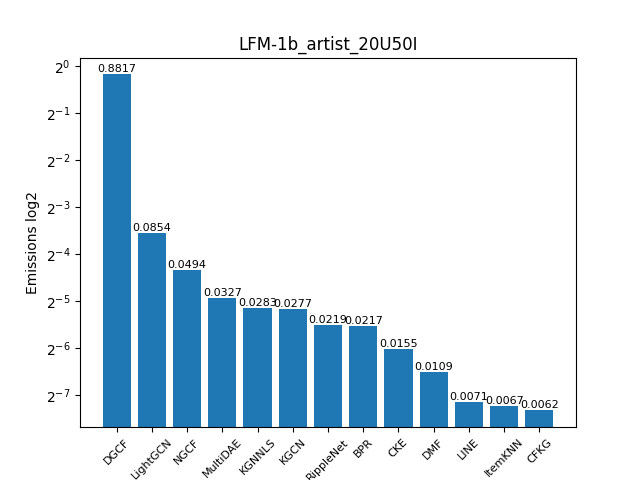
\includegraphics[width=\linewidth, trim=0 0 0 0]{images/emissions_LFM-1b_artist_20U50I.png} &
        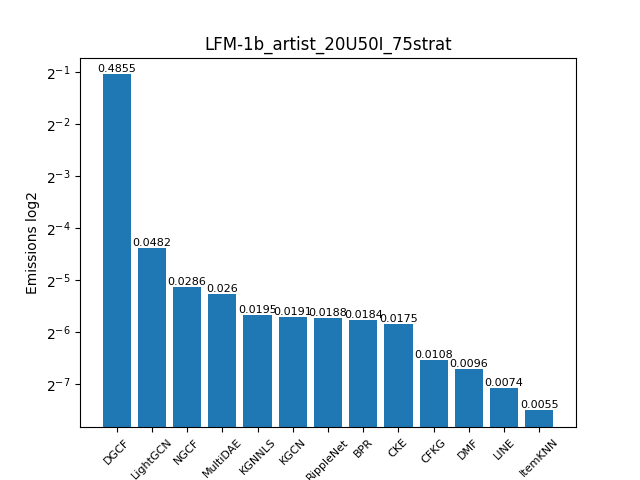
\includegraphics[width=\linewidth, trim=0 0 0 0]{images/emissions_LFM-1b_artist_20U50I_75strat.png} \\
        \hline
        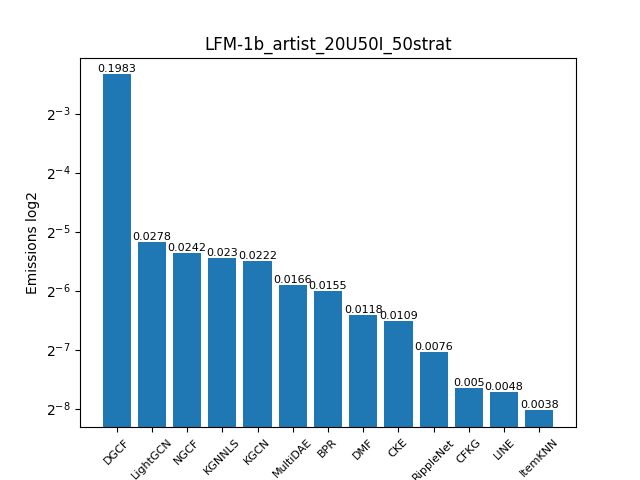
\includegraphics[width=\linewidth, trim=0 0 0 0]{images/emissions_LFM-1b_artist_20U50I_50strat.png} &
        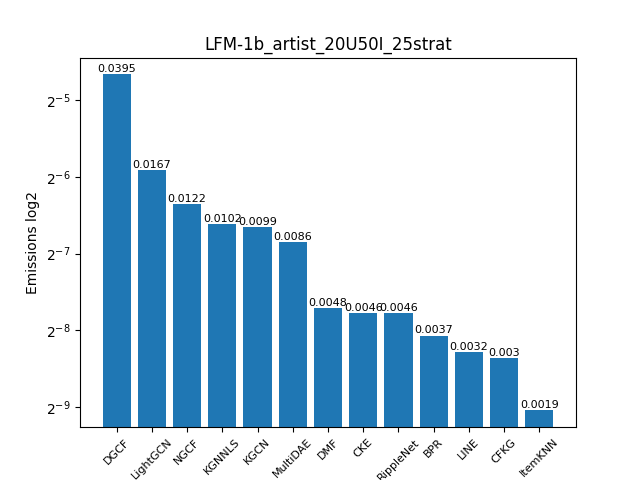
\includegraphics[width=\linewidth, trim=0 0 0 0]{images/emissions_LFM-1b_artist_20U50I_25strat.png} \\
        \hline
    \end{tabularx}
    \caption{Emissioni di CO2 per i vari dataset LFM-1b}
    \label{tab:emissions_info}
\end{table}

\noindent Si può subito notare come DGCF è il modello che emette più CO2 in assoluto.
In particolare con il dataset al 100\% e al 75\% DGCF emette circa 10 volte di più rispetto a LightGCN (il secondo per emissioni)
mentre con il dataset al 50\% emette circa 7 volte di più e con il dataset al 25\% emette circa 2 volte di più (sempre rispetto a LightGCN).
LightGCN e NCFG sono rispettivamente il secondo e il terzo modello che emettono più CO2.
Questi due modelli sono di tipo general, ma nonostante ciò emettono di più rispetto ad altri di tipo knowledge-aware, come per esempio il KGCN.
In generale possiamo vedere che ItemKNN,LINE e CFKG sono i modelli che emettono meno.
Per LINE e ItemKNN questo era abbastanza prevedibile in quanto modelli di tipo General. Interessante invece notare come CFKG, di tipo knowledge-aware, emetta meno di altri modelli di tipo General

\paragraph{MovieLens-10M\_50U10I} \textcolor{white}{.} \\
\begin{figure}[H]
    \centering
    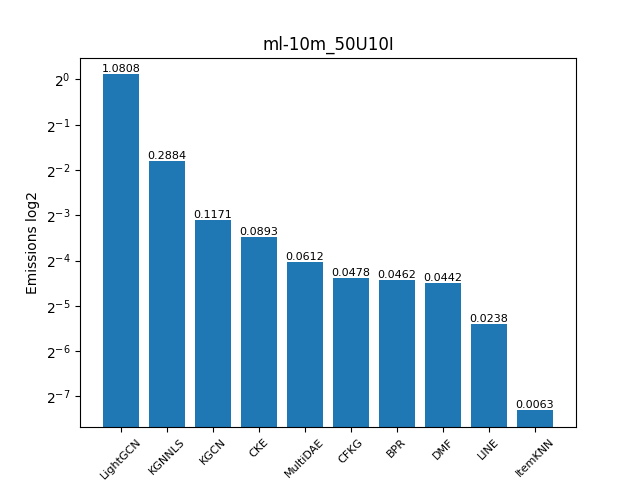
\includegraphics[scale=0.75]{images/emissions_ml-10m_50U10I.png}
    \caption{Emissioni di CO2 per il dataset MovieLens-10M\_50U10I}
\end{figure}

\noindent Si può subito notare come DGCF è il modello che emette più CO2 in assoluto.
In particolare con il dataset al 100\% e al 75\% DGCF emette circa 10 volte di più rispetto a LightGCN (il secondo per emissioni)
mentre con il dataset al 50\% emette circa 7 volte di più e con il dataset al 25\% emette circa 2 volte di più (sempre rispetto a LightGCN).
LightGCN e NCFG sono rispettivamente il secondo e il terzo modello che emettono più CO2.
Questi due modelli sono di tipo general, ma nonostante ciò emettono di più rispetto ad altri di tipo knowledge-aware, come per esempio il KGCN.
In generale possiamo vedere che ItemKNN,LINE e CFKG sono i modelli che emettono meno.
Per LINE e ItemKNN questo era abbastanza prevedibile in quanto modelli di tipo General. Interessante invece notare come CFKG, di tipo knowledge-aware, emetta meno di altri modelli di tipo General

\subsubsection{Trade-off}

In questa sezione verranno analizzati i trade-off tra le varie metriche di valutazione e le emissioni di CO2 analizzando un dataset per volta.

\paragraph{LFM-1b\_artist\_20U50I} \textcolor{white}{.} \\
\begin{table}[H]
    \centering
    \footnotesize
    \setlength\tabcolsep{0pt}
    \begin{tabularx}{\textwidth}{|X|X|}
        \hline
        \includegraphics[width=\linewidth, trim=0 0 0 0]{images/recall@10\_LFM-1b\_artist_20U50I.png} &
        \includegraphics[width=\linewidth, trim=0 0 0 0]{images/ndcg@10\_LFM-1b\_artist_20U50I.png} \\
        \hline
        \includegraphics[width=\linewidth, trim=0 0 0 0]{images/giniindex@10\_LFM-1b\_artist_20U50I.png} &
        \includegraphics[width=\linewidth, trim=0 0 0 0]{images/averagepopularity@10\_LFM-1b\_artist_20U50I.png} \\
        \hline
    \end{tabularx}
    \caption{Trade-off con il dataset LFM-1b\_artist\_20U50I}
    \label{tab:emissions_info}
\end{table}

\noindent Come già visto precedentemente, DGCF è il modello che emette di più. Nonostante ciò possiamo notare che per la recall e l'ndcg le sue performance risultano peggiori rispetto ad algoritmi più semplici come l'ItemKNN che risulta essere uno degli algoritmi che emette meno e performa meglio in queste metriche.
Per quanto riguarda il Gini Index possiamo notare che DGCF si comporta meglio di molti altri modelli ma l'ItemKNN e LINE risultano essere migliori di quest'ultimo. LINE è il miglior algoritmo.
Infine, per quanto riguarda l'Average Popularity, anche in questo caso possiamo notare anche che DGCF performa meglio di altri modelli, ma LINE risulta il miglior in assoluto ed è uno degli algoritmi che emette meno.

\paragraph{LFM-1b\_artist\_20U50I\_75strat} \textcolor{white}{.} \\
\begin{table}[H]
    \centering
    \footnotesize
    \setlength\tabcolsep{0pt}
    \begin{tabularx}{\textwidth}{|X|X|}
        \hline
        \includegraphics[width=\linewidth, trim=0 0 0 0]{images/recall@10\_LFM-1b\_artist_20U50I\_75strat.png} &
        \includegraphics[width=\linewidth, trim=0 0 0 0]{images/ndcg@10\_LFM-1b\_artist_20U50I\_75strat.png} \\
        \hline
        \includegraphics[width=\linewidth, trim=0 0 0 0]{images/giniindex@10\_LFM-1b\_artist_20U50I\_75strat.png} &
        \includegraphics[width=\linewidth, trim=0 0 0 0]{images/averagepopularity@10\_LFM-1b\_artist_20U50I\_75strat.png} \\
        \hline
    \end{tabularx}
    \caption{Trade-off con il dataset LFM-1b\_artist\_20U50I\_75strat}
    \label{tab:emissions_info}
\end{table}

\noindent Come già visto precedentemente, DGCF è il modello che emette di più. Nonostante ciò possiamo notare che per la recall e l'ndcg le sue performance risultano peggiori rispetto ad algoritmi più semplici come l'ItemKNN che risulta essere uno degli algoritmi che emette meno e performa meglio in queste metriche.
Per quanto riguarda il Gini Index possiamo notare che DGCF si comporta meglio di molti altri modelli ma l'ItemKNN e LINE risultano essere migliori di quest'ultimo. ItemKNN è il miglior algoritmo.
Infine, per quanto riguarda l'Average Popularity, anche in questo caso possiamo notare anche che DGCF performa meglio di altri modelli, ma LINE risulta il miglior in assoluto ed è uno degli algoritmi che emette meno.

\paragraph{LFM-1b\_artist\_20U50I\_50strat} \textcolor{white}{.} \\
\begin{table}[H]
    \centering
    \footnotesize
    \setlength\tabcolsep{0pt}
    \begin{tabularx}{\textwidth}{|X|X|}
        \hline
        \includegraphics[width=\linewidth, trim=0 0 0 0]{images/recall@10\_LFM-1b\_artist_20U50I\_50strat.png} &
        \includegraphics[width=\linewidth, trim=0 0 0 0]{images/ndcg@10\_LFM-1b\_artist_20U50I\_50strat.png} \\
        \hline
        \includegraphics[width=\linewidth, trim=0 0 0 0]{images/giniindex@10\_LFM-1b\_artist_20U50I\_50strat.png} &
        \includegraphics[width=\linewidth, trim=0 0 0 0]{images/averagepopularity@10\_LFM-1b\_artist_20U50I\_50strat.png} \\
        \hline
    \end{tabularx}
    \caption{Trade-off con il dataset LFM-1b\_artist\_20U50I\_50strat}
    \label{tab:emissions_info}
\end{table}


\noindent Come già visto precedentemente, DGCF è il modello che emette di più. Nonostante ciò possiamo notare che per la recall e l'ndcg le sue performance risultano peggiori rispetto ad altri algoritmi che emettono meno come CKE e CKFG(anch'essi di tipo Knowledge-Aware)..
Per quanto riguarda il Gini Index possiamo notare che DGCF si comporta meglio di molti altri modelli ma l'ItemKNN risulta essere migliore di quest'ultimo ed il migliore in assoluto.
Infine, per quanto riguarda l'Average Popularity, anche in questo caso possiamo notare anche che DGCF performa meglio di altri modelli, ma LINE risulta il miglior in assoluto ed è uno degli algoritmi che emette meno.

\paragraph{LFM-1b\_artist\_20U50I\_25strat} \textcolor{white}{.} \\
\begin{table}[H]
    \centering
    \footnotesize
    \setlength\tabcolsep{0pt}
    \begin{tabularx}{\textwidth}{|X|X|}
        \hline
        \includegraphics[width=\linewidth, trim=0 0 0 0]{images/recall@10\_LFM-1b\_artist_20U50I\_25strat.png} &
        \includegraphics[width=\linewidth, trim=0 0 0 0]{images/ndcg@10\_LFM-1b\_artist_20U50I\_25strat.png} \\
        \hline
        \includegraphics[width=\linewidth, trim=0 0 0 0]{images/giniindex@10\_LFM-1b\_artist_20U50I\_25strat.png} &
        \includegraphics[width=\linewidth, trim=0 0 0 0]{images/averagepopularity@10\_LFM-1b\_artist_20U50I\_25strat.png} \\
        \hline
    \end{tabularx}
    \caption{Trade-off con il dataset LFM-1b\_artist\_20U50I\_25strat}
    \label{tab:emissions_info}
\end{table}

\noindent Come già visto precedentemente, DGCF è il modello che emette di più. Nonostante ciò possiamo notare che per la recall e l'ndcg le sue performance risultano peggiori rispetto ad altri algoritmi che emettono meno come CKE e CKFG (anch'essi di tipo Knowledge-Aware).
Per quanto riguarda il Gini Index possiamo notare che DGCF si comporta meglio di molti altri modelli ma l'ItemKNN risulta essere di quest'ultimo migliore ed il migliore in assoluto.
Infine, per quanto riguarda l'Average Popularity, in questo caso possiamo notare anche che DGCF è uno dei peggiori mentre ItemKNN risulta il miglior in assoluto ed è l'algoritmo che emette meno.

\paragraph{MovieLens-10M\_50U10I} \textcolor{white}{.} \\
\begin{table}[H]
    \centering
    \footnotesize
    \setlength\tabcolsep{0pt}
    \begin{tabularx}{\textwidth}{|X|X|}
        \hline
        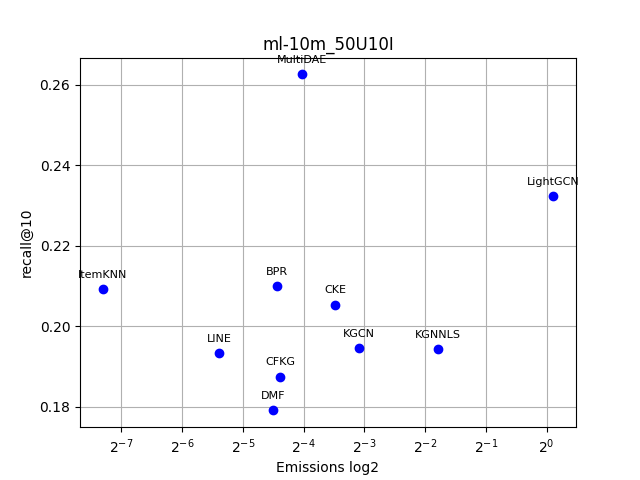
\includegraphics[width=\linewidth, trim=0 0 0 0]{images/recall@10_ml-10m_50U10I.png} &
        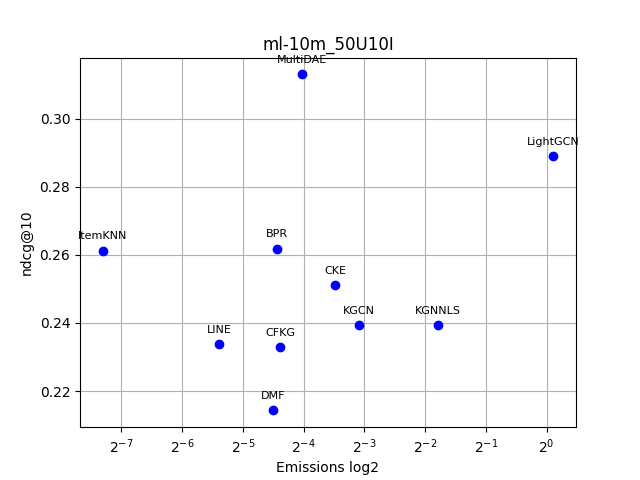
\includegraphics[width=\linewidth, trim=0 0 0 0]{images/ndcg@10_ml-10m_50U10I.png} \\
        \hline
        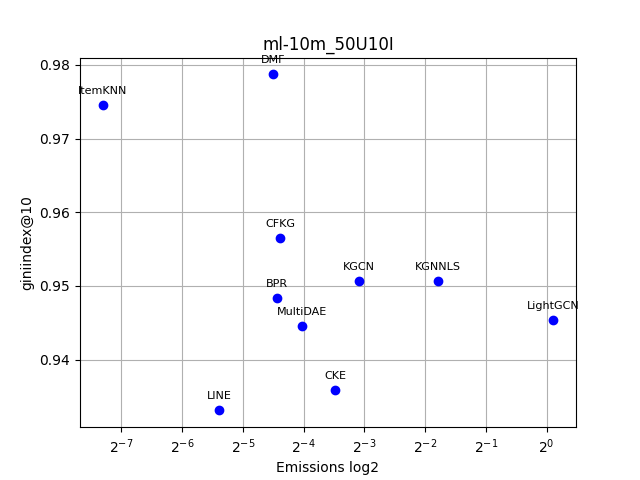
\includegraphics[width=\linewidth, trim=0 0 0 0]{images/giniindex@10_ml-10m_50U10I.png} &
        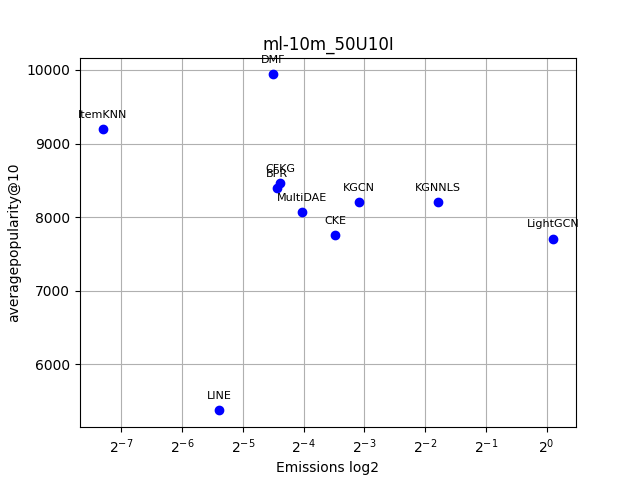
\includegraphics[width=\linewidth, trim=0 0 0 0]{images/averagepopularity@10_ml-10m_50U10I.png} \\
        \hline
    \end{tabularx}
    \caption{Trade-off con il datasetMovieLens-10M\_50U10I}
    \label{tab:emissions_info}
\end{table}


\noindent LightGCN è l'algoritmo che emette di più, osservando i valori da 5 a circa 180 volte rispetto agli altri modelli.
Emissioni cosi alte non sono però giustificate. Nelle metriche di recall e ndcg LightGCN è il secondo migliore, ma la differenza rispetto al primo è molto bassa e quindi non giustifica emissioni così alte.
ItemKNN si conferma uno dei migliori algoritmi per queste due metriche in quanto emette meno ed è uno dei più performanti.
Per quanto riguarda le metriche di Gini Index e Average Popularity possiamo notare che LightGCN è uno di migliori, ma anche in questo caso la differenza rispetto ad altri modelli non giustifica emissioni così alte. ItemKNN si conferma con il secondo peggior modello come punteggi. Line risulta essere il migliore in quanto è il secondo per basse emissioni ed ottiene i punteggi migliori. 

\subsubsection{Conclusioni}

Si può facilmente notare come il trade-off emissioni-performance sia decisamente a svantaggio dell'DGCF. Infatti, a fronte di emissioni molto elevate, le performance risultato spesso essere peggiori di modelli molto più semplici.
Con i due dataset più grandi possiamo notare come in generale ItemKNN risulti essere uno degli algoritmi con il miglior trade-off emissioni-performance nelle metriche di ranking, mentre LINE risulta essere il migliore nelle metriche di popolarità e equità nelle distribuzioni.
Al diminuire della dimensione del dataset DGCF comincia a comportarsi meglio nelle metriche di popolarità e equità, ma le sue emissioni rimangono sempre molto alte e non giustificano una possibile scelta di questo modello.
ItemKNN comincia a non performare bene nelle metriche di ranking, mentre migliora nelle metriche di popolarità e equità, arrivando anche a risultare il migliore




\subsection{Addestramento sostenibile}
\subsubsection{Parte esplorativa}
\paragraph{Primo esperimento} \textcolor{white}{.} \\
\begin{table}[H]
    \centering
    \footnotesize
    \setlength\tabcolsep{0pt}
    \begin{tabularx}{\textwidth}{|X|X|}
        \hline
        \textbf{Criterio classico} & \textbf{Criterio modificato} \\
        \hline
        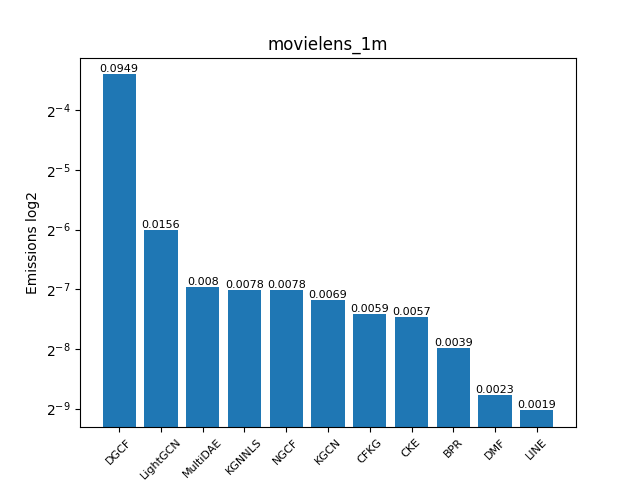
\includegraphics[width=\linewidth, trim=0 0 0 0]{images/emissions_movielens_1m_earlyClassic.png} &
        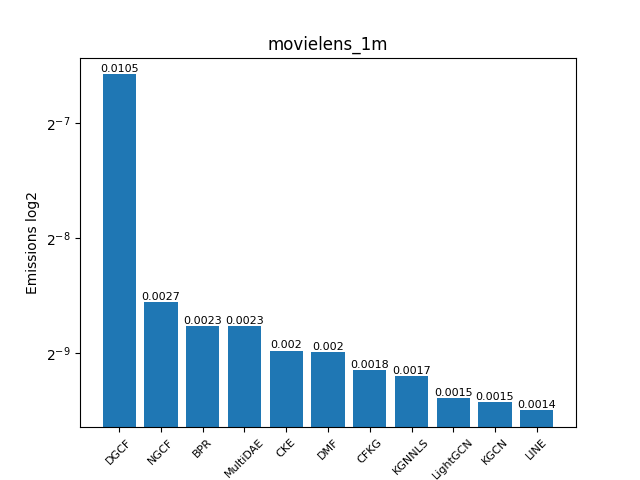
\includegraphics[width=\linewidth, trim=0 0 0 0]{images/emissions_movielens_1m_earlyModified.png} \\
        \hline
    \end{tabularx}
    \caption{Emissioni con criterio classico e modificato}
    \label{tab:emissions_info}
\end{table}

\noindent Si può dunque chiaramente notare come usando il nuovi criterio di early stopping le emissioni siano molto più basse rispetto al criterio classico.

\begin{table}[H]
    \centering
    \resizebox{\textwidth}{!}{
    \begin{tabular}{|c|c|c|c|c|}
        \hline
        \textbf{Modello} & \textbf{Emissioni criterio classico (g)} & \textbf{Emissioni criterio nuovo (g)} & \textbf{Riduzione} & \textbf{\% riduzione emissioni} \\
        \hline
        BPR & 3.9484 & 2.3033 & 1.6451 & 41.6647 \\
        \hline
        CKFG & 5.881 & 1.767 & 4.114 & 69.9418 \\
        \hline
        CKE & 5.68394 & 1.9837 & 3.70024 & 65.09955 \\
        \hline
        DMF & 2.2927 & 1.9667 & 0.326 & 14.2158 \\
        \hline
        KGCN & 6.8754 & 1.454 & 5.4214 & 78.8522 \\
        \hline
        KGNNLS & 7.763 & 1.70177 & 6.0613 & 78.0785 \\
        \hline
        LINE & 1.9128 & 1.3831 & 0.5297 & 27.6935 \\
        \hline
        MultiDAE & 8.0303 & 2.29608 & 5.73422 & 71.40737 \\
        \hline
        LightGCN & 15.626 & 1.4926 & 14.1334 & 90.4481 \\
        \hline
        NGCF & 7.7582 & 2.6601 & 5.0981 & 65.7126 \\
        \hline
        DGCF & 94.903 & 10.4625 & 84.4405 & 88.9756 \\
        \hline
    \end{tabular}
    }
    \caption{Confronto delle emissioni}
\end{table}


\noindent Si può dunque notare come in generale la percentuale di riduzione delle emissioni è molto alta



\begin{figure}[H]
    \centering
    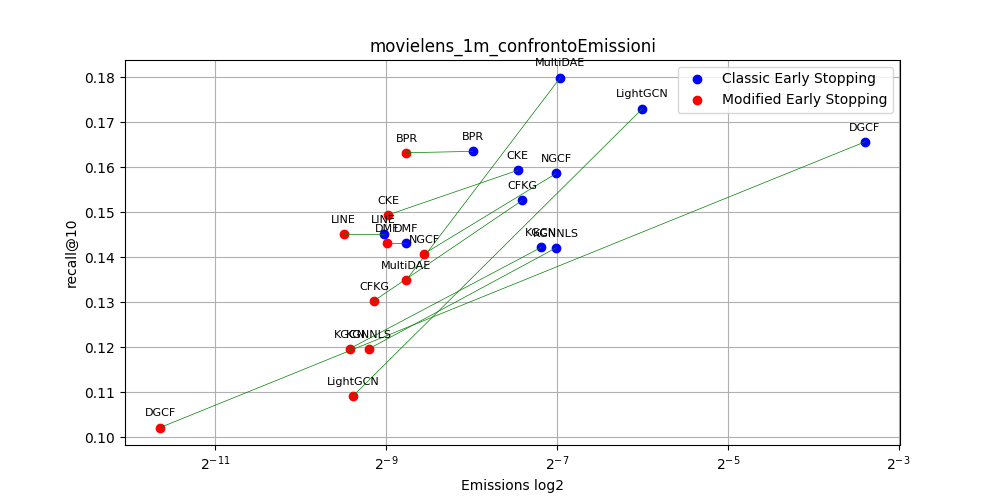
\includegraphics[width=\linewidth, trim=0 0 0 0]{images/recall@10_movielens_1m_comparison.png}
    \caption{Confronto score recall@10 con dataset MovieLens-1m}
    
\end{figure}

\begin{figure}[H]
    \centering
    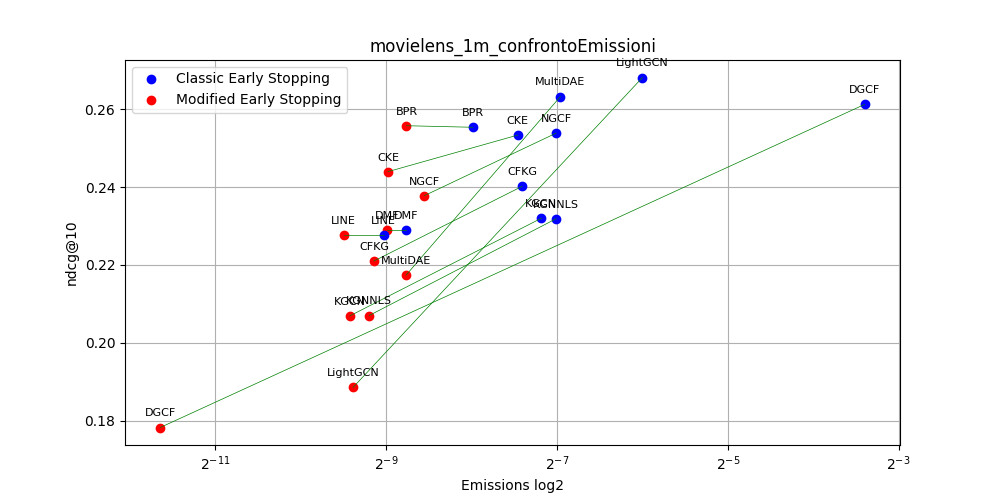
\includegraphics[width=\linewidth, trim=0 0 0 0]{images/ndcg@10_movielens_1m_comparison.png}
    \caption{Confronto score ndcg@10 con dataset MovieLens-1m}
    
\end{figure}

\begin{figure}[H]
    \centering
    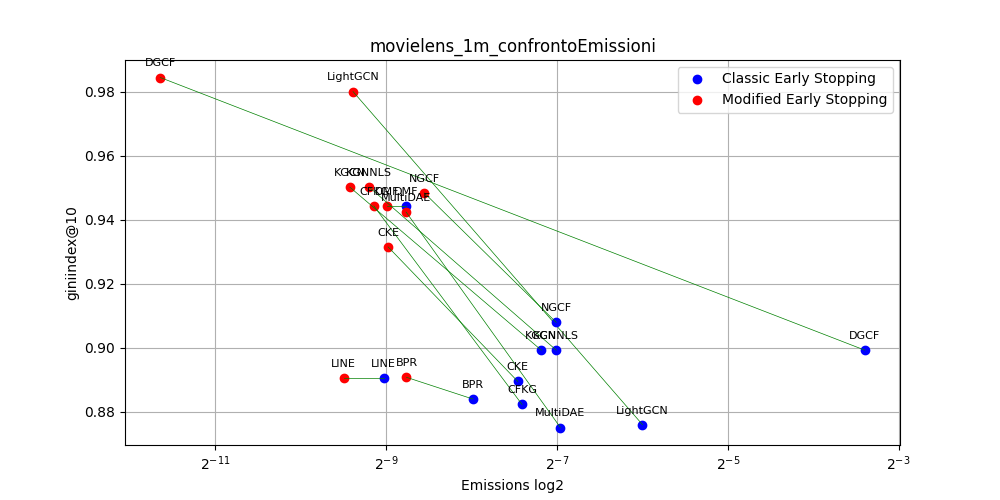
\includegraphics[width=\linewidth, trim=0 0 0 0]{images/giniindex@10_movielens_1m_comparison.png}
    \caption{Confronto score giniindex@10 con dataset MovieLens-1m}
\end{figure}

\begin{figure}[H]
    \centering
    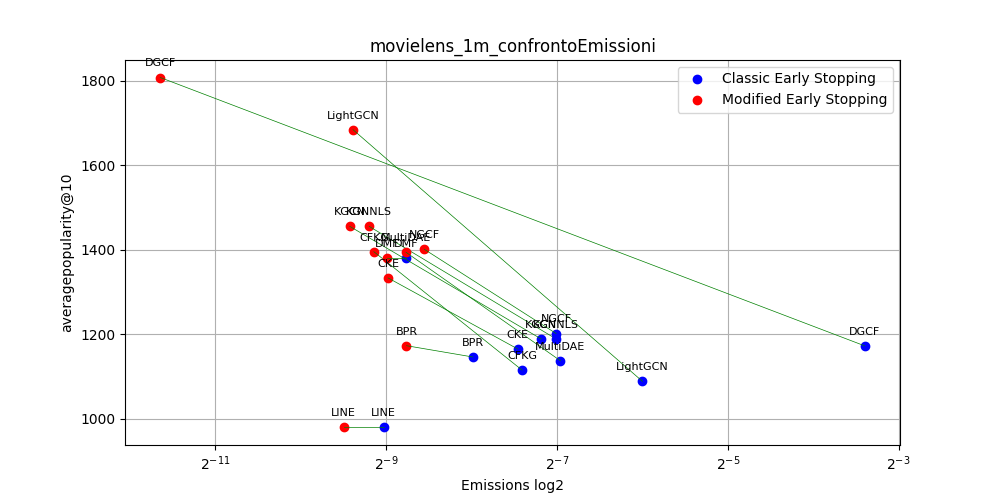
\includegraphics[width=\linewidth, trim=0 0 0 0]{images/averagepopularity@10_movielens_1m_comparison.png}
    \caption{Confronto score averagepopularity@10 con dataset MovieLens-1m}
\end{figure}





\begin{table}[H]
    \centering
    \resizebox{\textwidth}{!}{
        \begin{tabular}{|c|c|c|c|c|c|}
            \hline
            \textbf{Metrica} & \textbf{Modello} & \textbf{Score criterio classico} & \textbf{Score criterio nuovo} & \textbf{Riduzione} & \textbf{\% riduzione score} \\
            \hline
            \multirow{11}{*}{recall@10} & BPR & 0.1635 & 0.1632 & 0.0003 & 0.1835 \\ \cline{2-6}
                                         & CFKG & 0.1526 & 0.1303 & 0.0223 & 14.6134 \\ \cline{2-6}
                                         & CKE & 0.1593 & 0.1494 & 0.0099 & 6.2147 \\ \cline{2-6}
                                         & DMF & 0.1432 & 0.1432 & 0.0 & 0.0 \\ \cline{2-6}
                                         & KGCN & 0.1422 & 0.1197 & 0.0225 & 15.8228 \\ \cline{2-6}
                                         & KGNNLS & 0.1421 & 0.1197 & 0.0224 & 15.7635 \\ \cline{2-6}
                                         & LINE & 0.1451 & 0.1451 & 0.0 & 0.0 \\ \cline{2-6}
                                         & MultiDAE & 0.1799 & 0.1349 & 0.045 & 25.0139 \\ \cline{2-6}
                                         & LightGCN & 0.173 & 0.1092 & 0.0638 & 36.8786 \\ \cline{2-6}
                                         & NGCF & 0.1586 & 0.1408 & 0.0178 & 11.2232 \\ \cline{2-6}
                                         & DGCF & 0.1656 & 0.1022 & 0.0634 & 38.2850 \\ \cline{2-6}
            \hline
            \multirow{11}{*}{ndcg@10} & BPR & 0.2554 & 0.2558 & -0.0004 & -0.1566 \\ \cline{2-6}
                                       & CFKG & 0.2402 & 0.221 & 0.0192 & 7.9933 \\ \cline{2-6}
                                       & CKE & 0.2534 & 0.244 & 0.0094 & 3.7096 \\ \cline{2-6}
                                       & DMF & 0.2289 & 0.2289 & 0.0 & 0.0 \\ \cline{2-6}
                                       & KGCN & 0.232 & 0.2069 & 0.0251 & 10.819 \\ \cline{2-6}
                                       & KGNNLS & 0.2319 & 0.207 & 0.0249 & 10.737 \\ \cline{2-6}
                                       & LINE & 0.2277 & 0.2277 & 0.0 & 0.0 \\ \cline{2-6}
                                       & MultiDAE & 0.2633 & 0.2174 & 0.0459 & 17.433 \\ \cline{2-6}
                                       & LightGCN & 0.2682 & 0.1885 & 0.0797 & 29.717 \\ \cline{2-6}
                                       & NGCF & 0.2539 & 0.2378 & 0.0161 & 6.3411 \\ \cline{2-6}
                                       & DGCF & 0.2613 & 0.1782 & 0.0831 & 31.8025 \\ \cline{2-6}
            \hline
            \multirow{11}{*}{averagepopularity@10} & BPR & 1146.3572 & 1173.1199 & -26.7627 & -2.3346 \\ \cline{2-6}
                                                    & CFKG & 1115.4498 & 1395.6098 & -280.16 & -25.1163 \\ \cline{2-6}
                                                    & CKE & 1165.2413 & 1333.5153 & -168.274 & -14.4411 \\ \cline{2-6}
                                                    & DMF & 1379.7292 & 1379.7292 & 0.0 & 0.0 \\ \cline{2-6}
                                                    & KGCN & 1188.9582 & 1455.5651 & -266.6069 & -22.4236 \\ \cline{2-6}
                                                    & KGNNLS & 1188.8981 & 1455.58 & -266.6819 & -22.4310 \\ \cline{2-6}
                                                    & LINE & 979.498 & 979.498 & 0.0 & 0.0 \\ \cline{2-6}
                                                    & MultiDAE & 1137.4597 & 1394.0944 & -256.6347 & -22.5621 \\ \cline{2-6}
                                                    & LightGCN & 1088.741 & 1684.4149 & -595.6739 & -54.7122 \\ \cline{2-6}
                                                    & NGCF & 1201.8831 & 1401.4325 & -199.5494 & -16.6031 \\ \cline{2-6}
                                                    & DGCF & 1172.6874 & 1807.9828 & -635.2954 & -54.1743 \\ \cline{2-6}
            \hline
            \multirow{11}{*}{giniindex@10} & BPR & 0.8839 & 0.8907 & -0.0068 & -0.7693 \\ \cline{2-6}
                                            & CFKG & 0.8822 & 0.9443 & -0.0621 & -7.0392 \\ \cline{2-6}
                                            & CKE & 0.8894 & 0.9315 & -0.0421 & -4.7335 \\ \cline{2-6}
                                            & DMF & 0.9443 & 0.9443 & 0.0 & 0.0 \\ \cline{2-6}
                                            & KGCN & 0.8992 & 0.9502 & -0.051 & -5.6717 \\ \cline{2-6}
                                            & KGNNLS & 0.8992 & 0.9502 & -0.051 & -5.6717 \\ \cline{2-6}
                                            & LINE & 0.8904 & 0.8904 & 0.0 & 0.0 \\ \cline{2-6}
                                            & MultiDAE & 0.875 & 0.9424 & -0.0674 & -7.7029 \\ \cline{2-6}
                                            & LightGCN & 0.8759 & 0.9801 & -0.1042 & -11.8963 \\ \cline{2-6}
                                            & NGCF & 0.9079 & 0.9484 & -0.0405 & -4.4608 \\     \cline{2-6}
                                            & DGCF & 0.8992 & 0.9845 & -0.0853 & -9.4862 \\ \cline{2-6}
            \hline
        \end{tabular}
    }
    \caption{Confronto degli score tra criteri e modelli}
    \label{tab:confronto-score}
\end{table}


\begin{figure}[H]
    \centering
     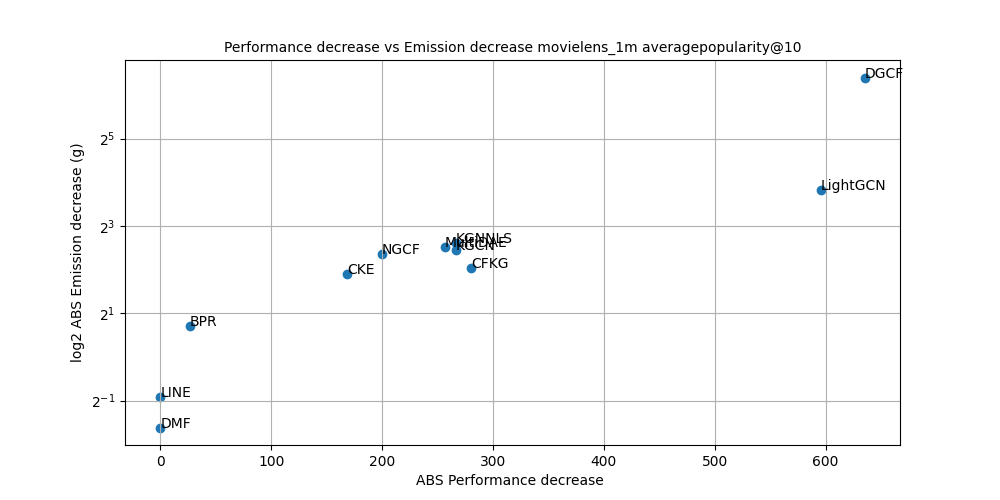
\includegraphics[width=\textwidth]{images/decrement_averagepopularity@10_movielens_1m.png}
    \caption{Decremento di averagepopularity@10}
\end{figure}

\begin{figure}[H]
    \centering
     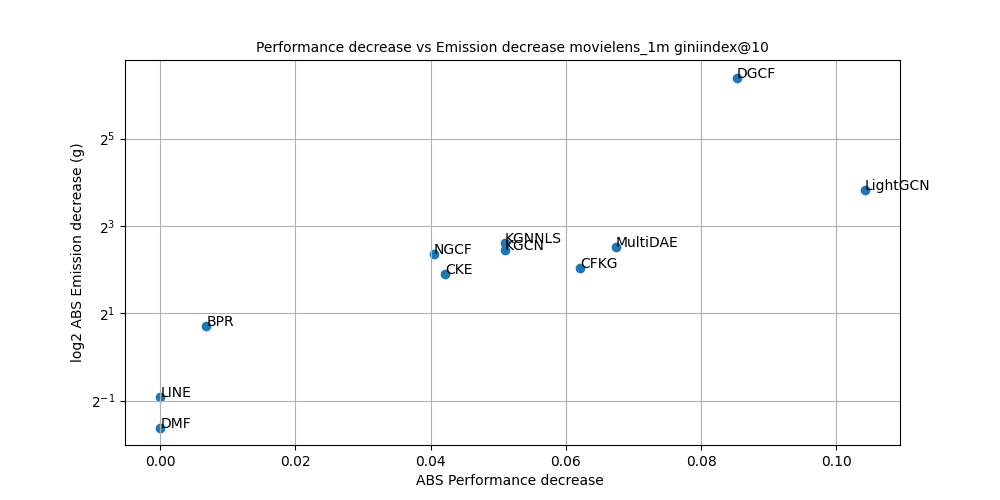
\includegraphics[width=\textwidth]{images/decrement_giniindex@10_movielens_1m.png}
    \caption{Decremento di giniindex@10}
\end{figure}

\begin{figure}[H]
    \centering
     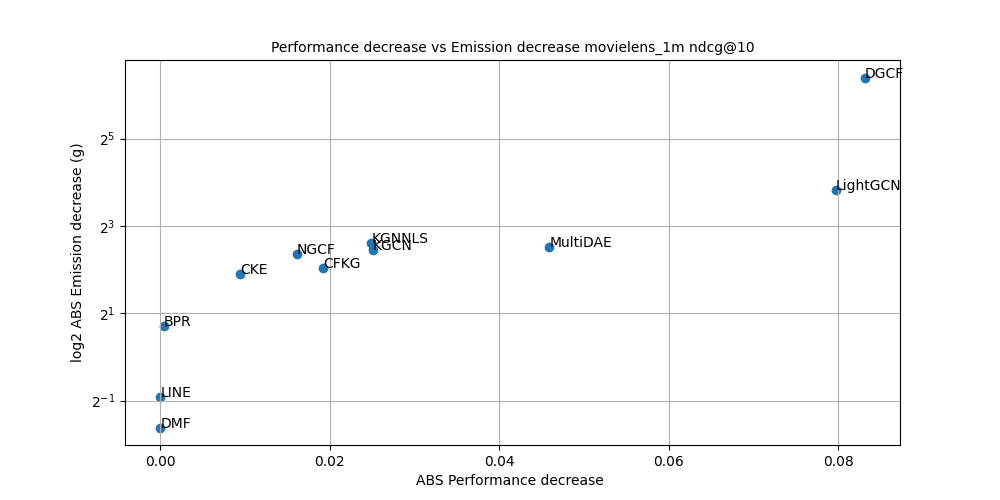
\includegraphics[width=\textwidth]{images/decrement_ndcg@10_movielens_1m.png}
    \caption{Decremento di ndcg@10}
\end{figure}

\begin{figure}[H]
    \centering
     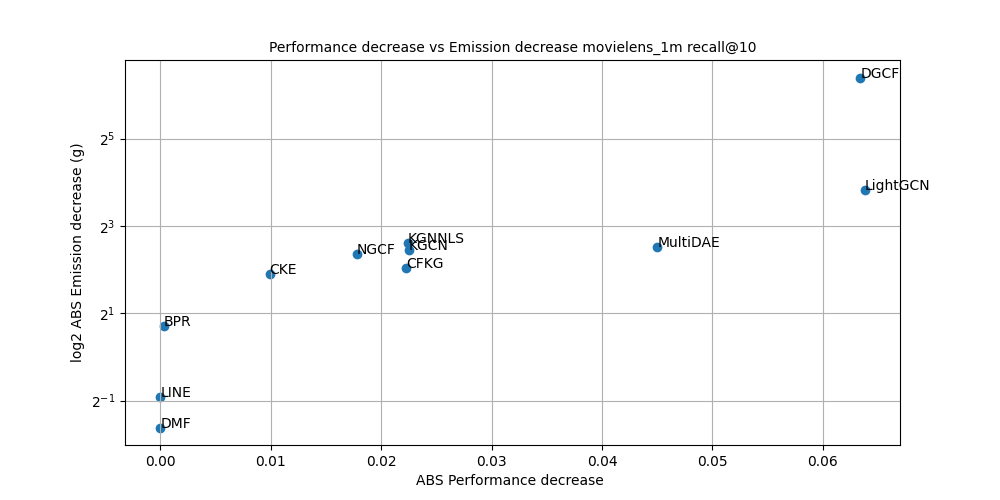
\includegraphics[width=\textwidth]{images/decrement_recall@10_movielens_1m.png}
    \caption{Decremento di recall@10}
\end{figure}


\noindent Per quanto riguarda giniindex e averagepopularity un punteggio più basso è migliore, mentre per recall e ndcg un punteggio più alto è migliore.
Ecco perchè la percentuale di riduzione degli score è negativa per giniindex e averagepopularity.

\noindent Confrontando le percentuali di riduzione delle emissioni e degli score si può notare la riduzione delle emissioni è molto più alta rispetto alla riduzione degli score.

\noindent BPR tende a mantenere le stesse perfomance con entrambi i criteri a fronte di emissioni molto più basse.
Possiamo notare come LINE e DMF non abbiano subito variazioni di score, mentre LightGCN e DGCF abbiano subito una riduzione molto alta (in percentuale comunque molto inferiore rispetto alla riduzione delle emissioni).
Probabilmente per LINE e DMF il criterio di early stopping classico ha portato ad eseguire qualche epoca in più ma che non ha portato a miglioramenti.

\paragraph{Secondo esperimento} \textcolor{white}{.} \\
\begin{table}[H]
    \centering
    \footnotesize
    \setlength\tabcolsep{0pt}
    \begin{tabularx}{\textwidth}{|X|X|}
        \hline
        \textbf{Criterio classico} & \textbf{Criterio modificato} \\
        \hline
        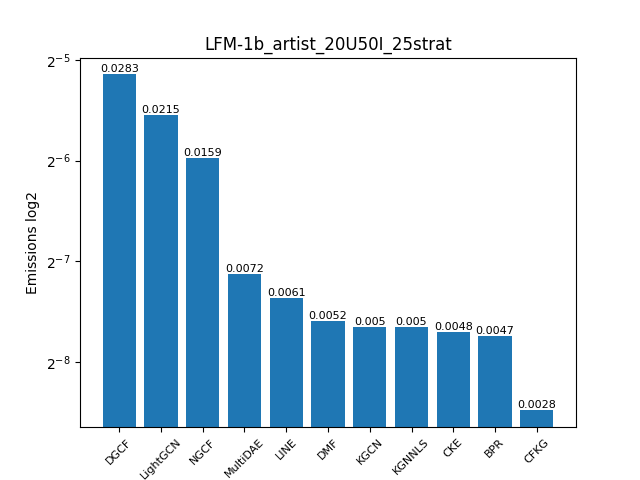
\includegraphics[width=\linewidth, trim=0 0 0 0]{images/emissions_LFM-1b_artist_20U50I_25strat_earlyClassic.png} &
        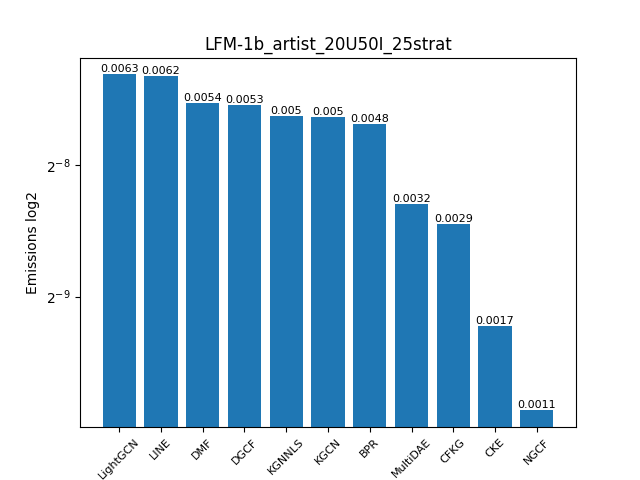
\includegraphics[width=\linewidth, trim=0 0 0 0]{images/emissions_LFM-1b_artist_20U50I_25strat_earlyModified.png} \\
        \hline
    \end{tabularx}
    \caption{Emissioni con criterio classico e modificato}
    \label{tab:emissions_info}
\end{table}



\begin{table}[H]
    \centering
    \resizebox{\textwidth}{!}{
    \begin{tabular}{|c|c|c|c|c|}
        \hline
        \textbf{Modello} & \textbf{Emissioni criterio classico (g)} & \textbf{Emissioni criterio nuovo (g)} & \textbf{Riduzione} & \textbf{\% riduzione emissioni} \\
        \hline
        BPR & 4.6785 & 4.8381 & -0.1596 & -3.4125 \\
        \hline
        CKFG & 2.8024 & 2.8539 & -0.0515 & -1.8368 \\
        \hline
        CKE & 4.8062 & 1.6694 & 3.1368 & 65.2659 \\
        \hline
        DMF & 5.1886 & 5.3978 & -0.2092 & -4.0321 \\
        \hline
        KGCN & 4.9718 & 5.0108 & -0.039 & -0.7863 \\
        \hline
        KGNNLS & 4.9701 & 5.0453 & -0.0752 & -1.5133 \\
        \hline
        LINE & 6.0602 & 6.2294 & -0.1692 & -2.7912 \\
        \hline
        MultiDAE & 7.1668 & 3.1731 & 3.9937 & 55.7245 \\
        \hline
        LightGCN & 21.4561 & 6.2812 & 15.1749 & 70.7256 \\
        \hline
        NGCF & 15.8887 & 1.0731 & 14.8156 & 93.2463 \\
        \hline
        DGCF & 28.2945 & 5.3468 & 22.9477 & 81.1035 \\
        \hline
    \end{tabular}
    }
    \caption{Confronto delle emissioni}
\end{table}


\noindent Il criterio più stringente mostra chiaramente come la riduzione delle emissioni sia inferiore rispetto al primo esperimento.
Per alcuni modelli vengono registrate addirittura delle variazioni negative, ovvero le emissioni sono aumentate rispetto al criterio classico. Questo potrebbe dipende da un picco di consumi dell'hardware in un certo momento, dovuto a qualche processo in background.
NGCF è l'unico modello in cui si registra un'aumento della percentuale di riduzione delle emissioni rispetto al primo esperimento.


\begin{figure}[H]
    \centering
    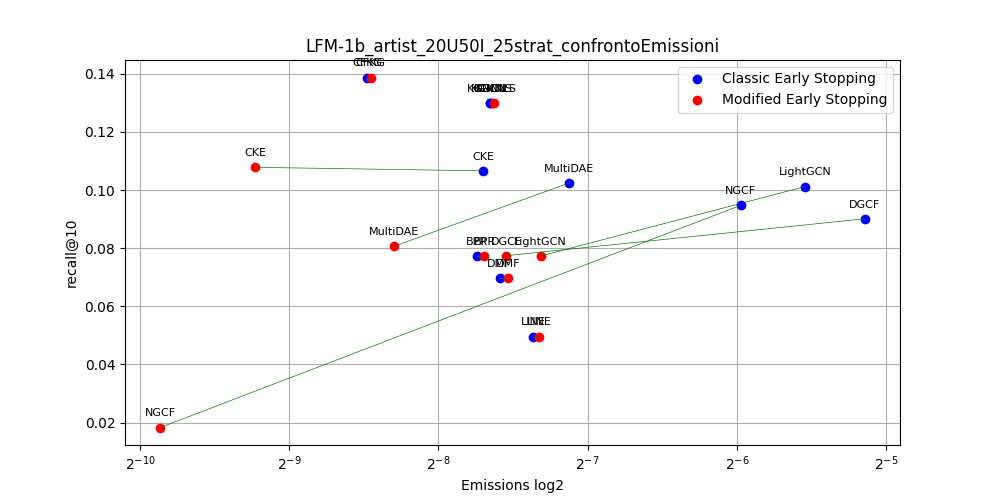
\includegraphics[width=\linewidth, trim=0 0 0 0]{images/recall@10_LFM-1b_artist_20U50I_25strat_comparison.png}
    \caption{Confronto score recall@10 con dataset LFM-1b\_artist\_20U50I\_25strat}
    
\end{figure}

\begin{figure}[H]
    \centering
    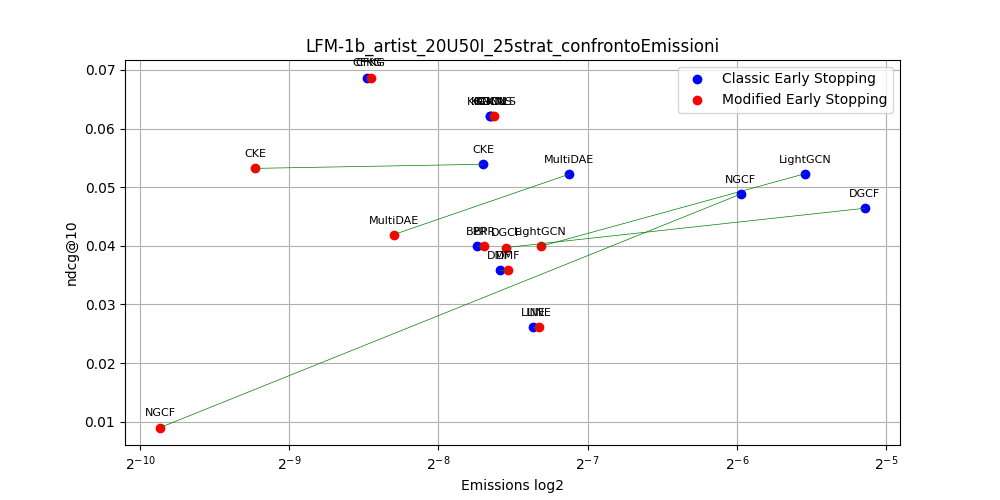
\includegraphics[width=\linewidth, trim=0 0 0 0]{images/ndcg@10_LFM-1b_artist_20U50I_25strat_comparison.png}
    \caption{Confronto score ndcg@10 con dataset LFM-1b\_artist\_20U50I\_25strat}
    
\end{figure}

\begin{figure}[H]
    \centering
    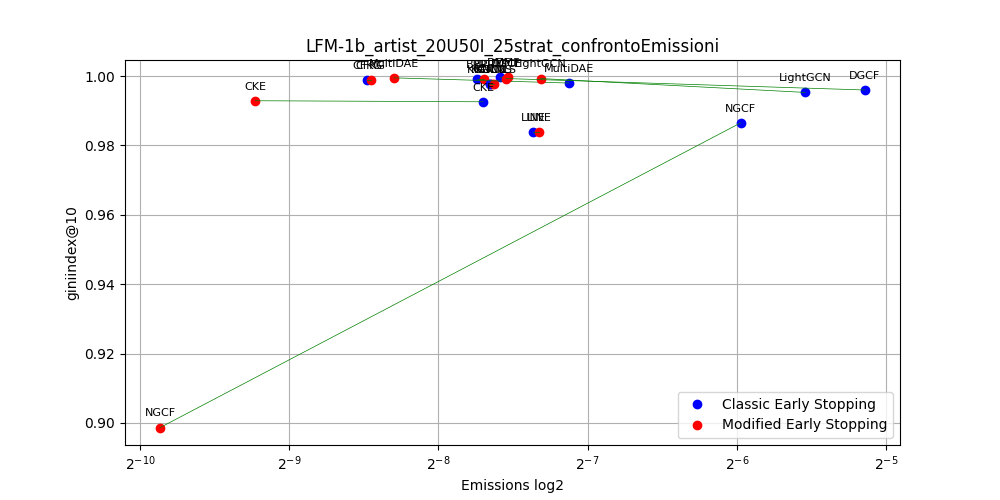
\includegraphics[width=\linewidth, trim=0 0 0 0]{images/giniindex@10_LFM-1b_artist_20U50I_25strat_comparison.png}
    \caption{Confronto score giniindex@10 con dataset LFM-1b\_artist\_20U50I\_25strat}
\end{figure}

\begin{figure}[H]
    \centering
    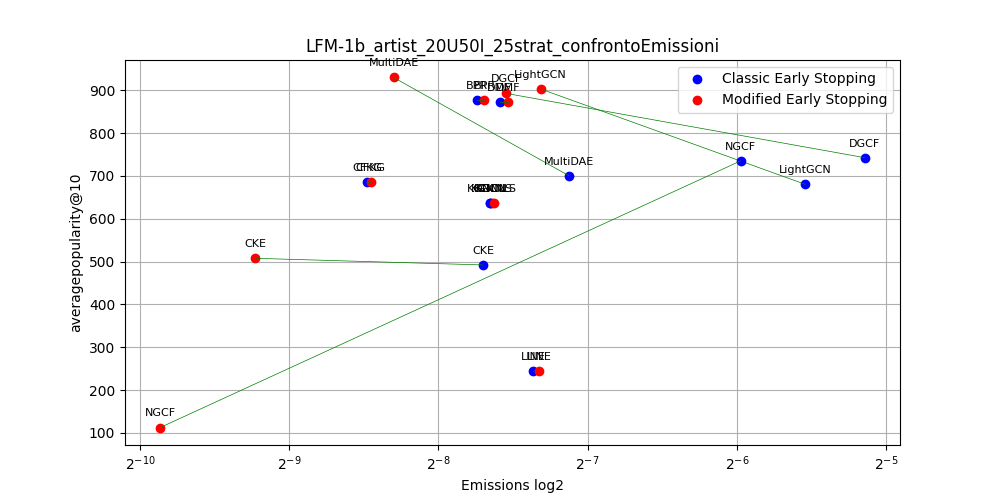
\includegraphics[width=\linewidth, trim=0 0 0 0]{images/averagepopularity@10_LFM-1b_artist_20U50I_25strat_comparison.png}
    \caption{Confronto score averagepopularity@10 con dataset LFM-1b\_artist\_20U50I\_25strat}
\end{figure}


\begin{table}[H]
    \centering
    \resizebox{\textwidth}{!}{
        \begin{tabular}{|c|c|c|c|c|c|}
            \hline
            \textbf{Metrica} & \textbf{Modello} & \textbf{Score criterio classico} & \textbf{Score criterio nuovo} & \textbf{Riduzione} & \textbf{\% riduzione score} \\
            \hline
            \multirow{11}{*}{recall@10} & BPR & 0.0772 & 0.0772 & 0.0 & 0.0 \\ \cline{2-6}
                                        & CFKG & 0.1387 & 0.1387 & 0.0 & 0.0 \\ \cline{2-6}
                                        & CKE & 0.1078 & 0.1066 & -0.0121 & -1.1257 \\ \cline{2-6}
                                        & DMF & 0.0698 & 0.0698 & 0.0 & 0.0 \\ \cline{2-6}
                                        & KGCN & 0.1299 & 0.1299 & 0.0 & 0.0 \\ \cline{2-6}
                                        & KGNNLS & 0.1299 & 0.1299 & 0.0 & 0.0 \\ \cline{2-6}
                                        & LINE & 0.0496 & 0.0496 & 0.0 & 0.0 \\ \cline{2-6}
                                        & MultiDAE & 0.0806 & 0.1024 & 0.0218 & 21.2891 \\ \cline{2-6}
                                        & LightGCN & 0.0773 & 0.1012 & 0.0239 & 23.6166 \\ \cline{2-6}
                                        & NGCF & 0.0183 & 0.0947 & 0.0764 & 80.6758 \\\cline{2-6}
                                        & DGCF & 0.0774 & 0.0901 & 0.0127 & 14.0954 \\ \cline{2-6}
            \hline
            \multirow{11}{*}{ndcg@10} & BPR & 0.04 & 0.04 & 0.0 & 0.0 \\ \cline{2-6}
                                      & CFKG & 0.0687 & 0.0687 & 0.0 & 0.0 \\ \cline{2-6}
                                      & CKE & 0.0532 & 0.0539 & 0.0007 & 1.2987 \\ \cline{2-6}
                                      & DMF & 0.0359 & 0.0359 & 0.0 & 0.0 \\ \cline{2-6}
                                      & KGCN & 0.0621 & 0.0621 & 0.0 & 0.0 \\ \cline{2-6}
                                      & KGNNLS & 0.0621 & 0.0621 & 0.0 & 0.0 \\ \cline{2-6}
                                      & LINE & 0.0261 & 0.0261 & 0.0 & 0.0 \\ \cline{2-6}
                                      & MultiDAE & 0.0419 & 0.0522 & 0.0103 & 19.7318 \\ \cline{2-6}
                                      & LightGCN & 0.0399 & 0.0523 & 0.0124 & 23.7094 \\ \cline{2-6}
                                      & NGCF & 0.009 & 0.0488 & 0.0398 & 81.5574 \\ \cline{2-6}
                                      & DGCF & 0.0397 & 0.0464 & 0.0067 & 14.4397 \\ \cline{2-6}
            \hline
            \multirow{11}{*}{averagepopularity@10} & BPR & 877.7191 & 877.7191 & 0.0 & 0.0 \\ \cline{2-6}
                                                  & CFKG & 686.1384 & 686.1384 & 0.0 & 0.0 \\ \cline{2-6}
                                                  & CKE & 507.6022 & 492.1156 & -15.4866 & -3.1469 \\ \cline{2-6}
                                                  & DMF & 872.5193 & 872.5193 & 0.0 & 0.0 \\ \cline{2-6}
                                                  & KGCN & 635.7879 & 635.7879 & 0.0 & 0.0 \\ \cline{2-6}
                                                  & KGNNLS & 635.7866 & 635.7866 & 0.0 & 0.0 \\\cline{2-6}
                                                  & LINE & 244.7699 & 244.7699 & 0.0 & 0.0 \\ \cline{2-6}
                                                  & MultiDAE & 929.5664 & 700.0905 & -229.4759 & -32.778 \\ \cline{2-6}
                                                  & LightGCN & 902.6965 & 680.2857 & -222.4108 & -32.6937 \\ \cline{2-6}
                                                  & NGCF & 112.7163 & 734.8359 & 622.1196 & 84.661 \\ \cline{2-6}
                                                  & DGCF & 892.5034 & 742.4452 & -150.0582 & -20.2114 \\ \cline{2-6}
            \hline
            \multirow{11}{*}{giniindex@10} & BPR & 0.9991 & 0.9991 & 0.0 & 0.0 \\ \cline{2-6}
                                            & CFKG & 0.9989 & 0.9989 & 0.0 & 0.0 \\ \cline{2-6}
                                            & CKE & 0.9929 & 0.9926 & -0.0003 & -0.0302 \\ \cline{2-6}
                                            & DMF & 0.9996 & 0.9996 & 0.0 & 0.0 \\ \cline{2-6}
                                            & KGCN & 0.9978 & 0.9978 & 0.0 & 0.0 \\ \cline{2-6}
                                            & KGNNLS & 0.9978 & 0.9978 & 0.0 & 0.0 \\ \cline{2-6}
                                            & LINE & 0.984 & 0.984 & 0.0 & 0.0 \\ \cline{2-6}
                                            & MultiDAE & 0.9995 & 0.998 & -0.0015 & -0.1503 \\ \cline{2-6}
                                            & LightGCN & 0.9993 & 0.9953 & -0.004 & -0.4019 \\ \cline{2-6}
                                            & NGCF & 0.8987 & 0.9865 & 0.0878 & 8.9002 \\ \cline{2-6}
                                            & DGCF & 0.9993 & 0.996 & -0.0033 & -0.3313 \\ \cline{2-6}
            \hline
        \end{tabular}
    }
    \caption{Confronto degli score tra criteri e modelli}
\end{table}




\begin{figure}[H]
    \centering
     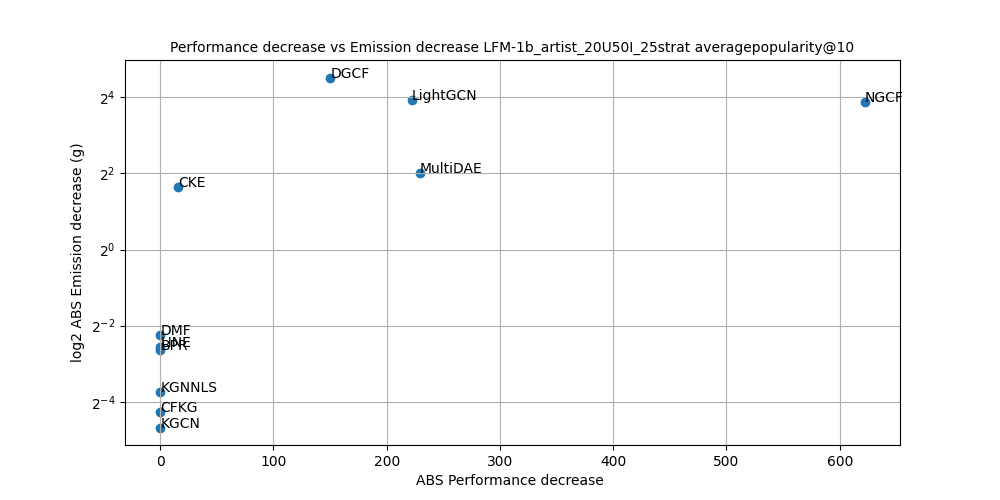
\includegraphics[width=\textwidth]{images/decrement_averagepopularity@10_LFM-1b_artist_20U50I_25strat.png}
    \caption{Decremento di averagepopularity@10}
\end{figure}

\begin{figure}[H]
    \centering
     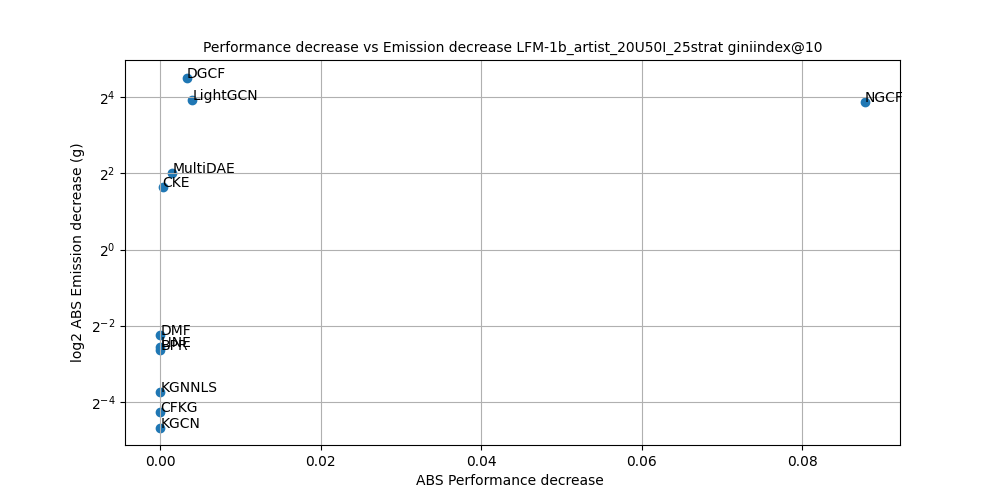
\includegraphics[width=\textwidth]{images/decrement_giniindex@10_LFM-1b_artist_20U50I_25strat.png}
    \caption{Decremento di giniindex@10}
\end{figure}

\begin{figure}[H]
    \centering
     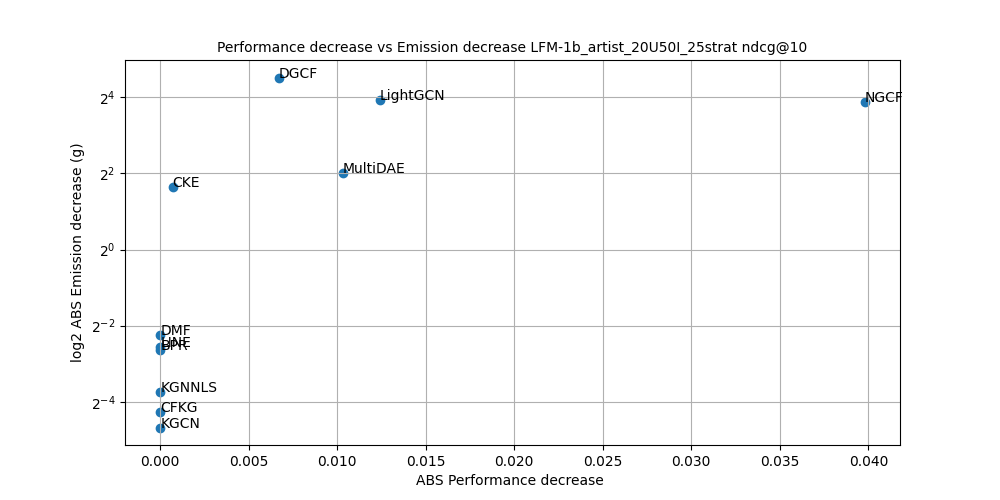
\includegraphics[width=\textwidth]{images/decrement_ndcg@10_LFM-1b_artist_20U50I_25strat.png}
    \caption{Decremento di ndcg@10}
\end{figure}

\begin{figure}[H]
    \centering
     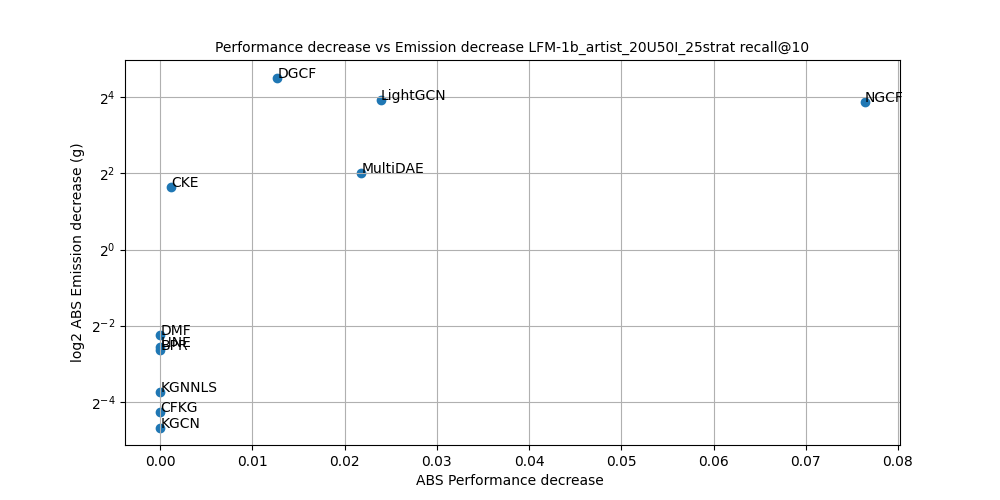
\includegraphics[width=\textwidth]{images/decrement_recall@10_LFM-1b_artist_20U50I_25strat.png}
    \caption{Decremento di recall@10}
\end{figure}


\noindent Si può chiaramente notare come gli algoritmi che prima avevano registrato un aumento delle emissioni abbiano le stesse performance ad ogni metrica.
Questo è un chiaro segno che in questo caso gli algoritmi in entrambi i casi abbiano terminato l'esecuzione con il criterio di early stopping classico e che le emissioni abbiano subito un picco in un certo momento dovuto ad altri fattori.
Si può chiaramente notare come, rispetto al primo esperimento, tutti gli altri modelli, ad eccezione di NGCF, abbiano subito una riduzione delle performance molto più bassa rispetto al primo esperimento a fronte di riduzione di emissioni minori, a conferma che il criterio più stringente ha permesso a questi modelli di continuare l'addestramento e dunque essere allenati per più epoche.
Un anomalia si può notare per NGCF, che ha subito una riduzione delle performance molto alta rispetto al primo esperimento a fronte di una riduzione delle emissioni molto più alte. In entrambi i casi la differenza di errore è dell'ordine dei centesimi. Questo potrebbe essere dovuto al un dataset con diverse caratteristiche rispetto al precedente.

\paragraph{Terzo esperimento} \textcolor{white}{.} \\
\begin{table}[H]
    \centering
    \footnotesize
    \setlength\tabcolsep{0pt}
    \begin{tabularx}{\textwidth}{|X|X|}
        \hline
        \textbf{Criterio classico} & \textbf{Criterio modificato} \\
        \hline
        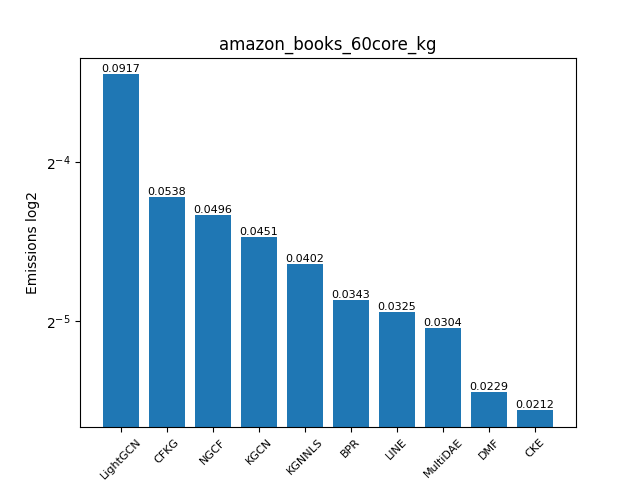
\includegraphics[width=\linewidth, trim=0 0 0 0]{images/emissions_amazon_books_60core_kg_earlyClassic.png} &
        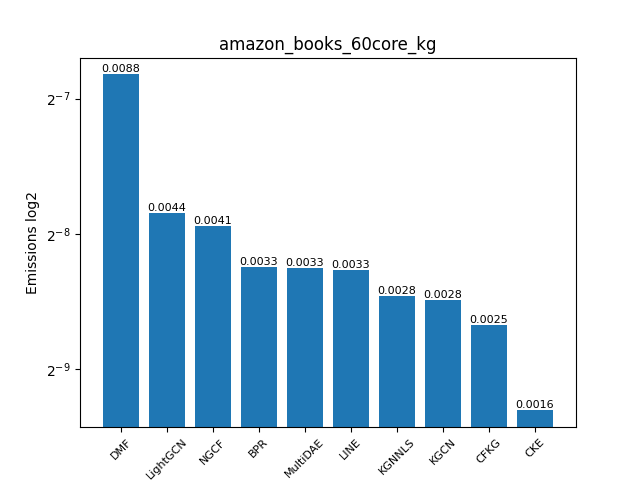
\includegraphics[width=\linewidth, trim=0 0 0 0]{images/emissions_amazon_books_60core_kg_earlyModified.png} \\
        \hline
    \end{tabularx}
    \caption{Emissioni con criterio classico e modificato}
    \label{tab:emissions_info}
\end{table}



\begin{table}[H]
    \centering
    \resizebox{\textwidth}{!}{
    \begin{tabular}{|c|c|c|c|c|}
        \hline
        \textbf{Modello} & \textbf{Emissioni criterio classico (g)} & \textbf{Emissioni criterio nuovo (g)} & \textbf{Riduzione} & \textbf{\% riduzione emissioni}\\
        \hline
        BPR & 34.3235 & 3.2958 & 31.0277 & 90.398\\
        \hline
        CKFG & 53.7798 & 2.4515 & 51.3283 & 95.4416\\
        \hline
        CKE & 21.1537 & 1.5824 & 19.5713 & 92.5194\\
        \hline
        DMF & 22.9403 & 8.8401 & 14.1002 & 61.4649\\
        \hline
        KGCN & 45.1294 & 2.7897 & 42.3397 & 93.8185\\
        \hline
        KGNNLS & 40.1533 & 2.8432 & 37.3101 & 92.9192\\
        \hline
        LINE & 32.5426 & 3.2539 & 29.2887 & 90.0011\\
        \hline
        MultiDAE & 30.3706 & 3.2749 & 27.0957 & 89.2169\\
        \hline
        LightGCN & 91.732 & 4.3526 & 87.3794 & 95.2551\\
        \hline
        NGCF & 49.55 & 4.0757 & 45.4743 & 91.7745\\
        \hline
    \end{tabular}
    }
    \caption{Confronto delle emissioni}
\end{table}

\noindent Come è possibile notare in questo caso la riduzione delle emissioni è molto alta per tutti i modelli, con valori che superano il 90\% per quasi tutti i modelli.


\begin{figure}[H]
    \centering
    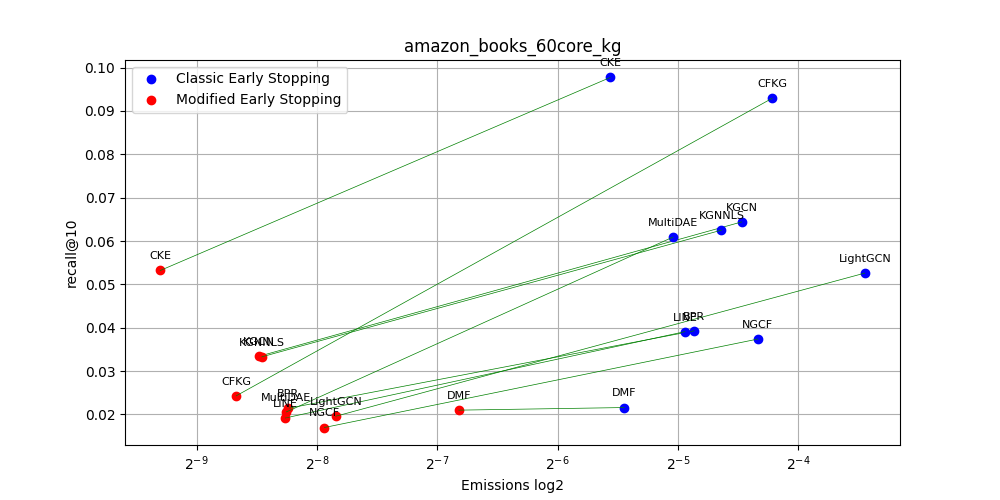
\includegraphics[width=\linewidth, trim=0 0 0 0]{images/recall@10_amazon_books_60core_kg_comparison.png}
    \caption{Confronto score recall@10 con dataset amazon\_books\_60core\_kg}
    
\end{figure}

\begin{figure}[H]
    \centering
    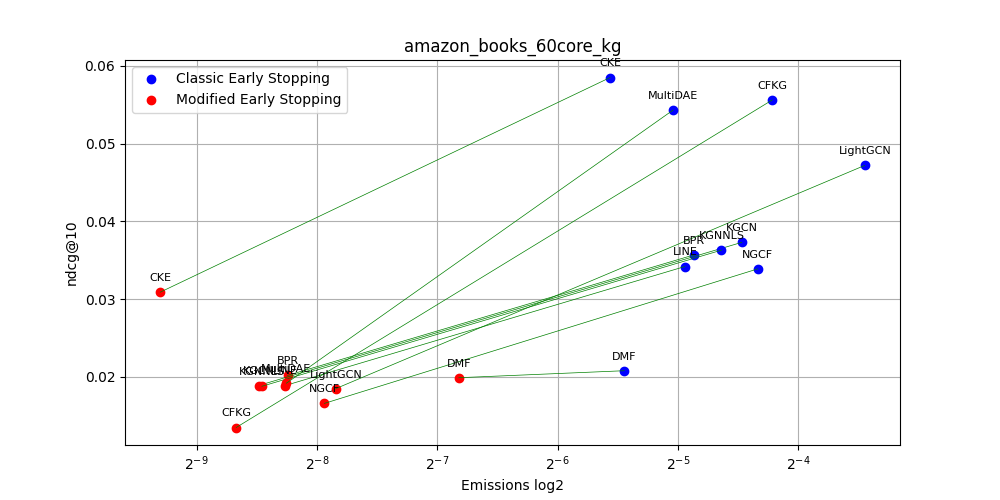
\includegraphics[width=\linewidth, trim=0 0 0 0]{images/ndcg@10_amazon_books_60core_kg_comparison.png}
    \caption{Confronto score ndcg@10 con dataset amazon\_books\_60core\_kg}
    
\end{figure}

\begin{figure}[H]
    \centering
    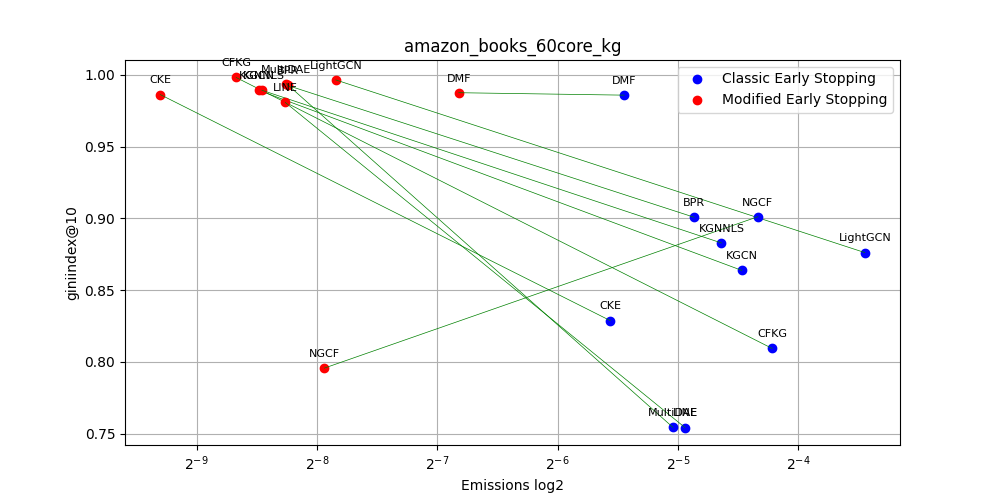
\includegraphics[width=\linewidth, trim=0 0 0 0]{images/giniindex@10_amazon_books_60core_kg_comparison.png}
    \caption{Confronto score giniindex@10 con dataset amazon\_books\_60core\_kg}
\end{figure}

\begin{figure}[H]
    \centering
    \includegraphics[width=\linewidth, trim=0 0 0 0]{images/averagepopularity@10_amazon_books_60core_kg_comparison.png}
    \caption{Confronto score averagepopularity@10 con dataset amazon\_books\_60core\_kg}
\end{figure}


\begin{table}[H]
    \centering
    \resizebox{\textwidth}{!}{
    \begin{tabular}{|c|c|c|c|c|c|}
        \hline
        \textbf{Metrica} & \textbf{Modello} & \textbf{Score criterio classico} & \textbf{Score criterio nuovo} & \textbf{Riduzione} & \textbf{\% riduzione score} \\ \hline
        \multirow{11}{*}{recall@10} & BPR & 0.0393 & 0.0214 & 0.0179 & 45.5471 \\ \cline{2-6} 
                                     & CFKG & 0.0929 & 0.0243 & 0.0686 & 73.8428 \\ \cline{2-6} 
                                     & CKE & 0.0977 & 0.0532 & 0.0445 & 45.5476 \\ \cline{2-6} 
                                     & DMF & 0.0216 & 0.021 & 0.0006 & 2.7778 \\ \cline{2-6} 
                                     & KGCN & 0.0644 & 0.0334 & 0.031 & 48.1366 \\ \cline{2-6} 
                                     & KGNNLS & 0.0625 & 0.0333 & 0.0292 & 46.72 \\ \cline{2-6} 
                                     & LINE & 0.0391 & 0.0192 & 0.0199 & 50.8951 \\ \cline{2-6} 
                                     & MultiDAE & 0.0609 & 0.0206 & 0.0403 & 66.1741 \\ \cline{2-6} 
                                     & LightGCN & 0.0526 & 0.0196 & 0.033 & 62.7376 \\ \cline{2-6} 
                                     & NGCF & 0.0374 & 0.017 & 0.0204 & 54.5455 \\ \cline{2-6} 
        \hline
        \multirow{11}{*}{ndcg@10} & BPR & 0.0357 & 0.0202 & 0.0155 & 43.4174 \\ \cline{2-6} 
                                   & CFKG & 0.0556 & 0.0135 & 0.0421 & 75.7194 \\ \cline{2-6} 
                                   & CKE & 0.0585 & 0.0309 & 0.0276 & 47.1795 \\ \cline{2-6} 
                                   & DMF & 0.0208 & 0.0199 & 0.0009 & 4.3269 \\ \cline{2-6} 
                                   & KGCN & 0.0373 & 0.0189 & 0.0184 & 49.3298 \\ \cline{2-6} 
                                   & KGNNLS & 0.0363 & 0.0188 & 0.0175 & 48.2094 \\ \cline{2-6} 
                                   & LINE & 0.0342 & 0.0189 & 0.0153 & 44.7368 \\ \cline{2-6} 
                                   & MultiDAE & 0.0543 & 0.0192 & 0.0351 & 64.6409 \\ \cline{2-6} 
                                   & LightGCN & 0.0472 & 0.0185 & 0.0287 & 60.8051 \\ \cline{2-6} 
                                   & NGCF & 0.0339 & 0.0166 & 0.0173 & 51.0324 \\ \cline{2-6} 
        \hline
        \multirow{11}{*}{avgpopularity@10} & BPR & 109.4148 & 220.0387 & -110.6239 & -101.1051 \\ \cline{2-6} 
                                            & CFKG & 122.3777 & 366.0359 & -243.6582 & -199.1034 \\ \cline{2-6} 
                                            & CKE & 117.927 & 229.8594 & -111.9324 & -94.9167 \\ \cline{2-6} 
                                            & DMF & 158.1008 & 156.3042 & 1.7966 & 1.1364 \\ \cline{2-6} 
                                            & KGCN & 140.0346 & 256.0119 & -115.9773 & -82.8205 \\ \cline{2-6} 
                                            & KGNNLS & 147.1768 & 256.0278 & -108.851 & -73.9593 \\ \cline{2-6} 
                                            & LINE & 58.1057 & 100.9865 & -42.8808 & -73.7979 \\ \cline{2-6} 
                                            & MultiDAE & 76.5618 & 207.1265 & -130.5647 & -170.535 \\ \cline{2-6} 
                                            & LightGCN & 105.7397 & 252.0464 & -146.3067 & -138.365 \\ \cline{2-6} 
                                            & NGCF & 113.2036 & 70.9028 & 42.3008 & 37.367 \\ \cline{2-6} 
        \hline
        \multirow{11}{*}{giniindex@10} & BPR & 0.9007 & 0.9926 & -0.0919 & -10.2032 \\ \cline{2-6} 
                                        & CFKG & 0.8093 & 0.9981 & -0.1888 & -23.3288 \\ \cline{2-6} 
                                        & CKE & 0.8287 & 0.9862 & -0.1575 & -19.0057 \\ \cline{2-6} 
                                        & DMF & 0.9858 & 0.9875 & -0.0017 & -0.1724 \\ \cline{2-6} 
                                        & KGCN & 0.8637 & 0.9892 & -0.1255 & -14.5305 \\ \cline{2-6} 
                                        & KGNNLS & 0.8828 & 0.9892 & -0.1064 & -12.0526 \\ \cline{2-6} 
                                        & LINE & 0.7542 & 0.9807 & -0.2265 & -30.0318 \\ \cline{2-6} 
                                        & MultiDAE & 0.7543 & 0.9938 & -0.2395 & -31.7513 \\ \cline{2-6} 
                                        & LightGCN & 0.8761 & 0.9964 & -0.1203 & -13.7313 \\ \cline{2-6} 
                                        & NGCF & 0.9011 & 0.7956 & 0.1055 & 11.7079 \\ \cline{2-6} 
        \hline
    \end{tabular}
    }
    \caption{Performance dei modelli su diverse metriche e dataset}
\end{table}


\begin{figure}[H]
    \centering
     \includegraphics[width=\textwidth]{images/decrement_averagepopularity@10_amazon_books_60core_kg.png}
    \caption{Decremento di averagepopularity@10}
\end{figure}

\begin{figure}[H]
    \centering
     \includegraphics[width=\textwidth]{images/decrement_giniindex@10_amazon_books_60core_kg.png}
    \caption{Decremento di giniindex@10}
\end{figure}

\begin{figure}[H]
    \centering
     \includegraphics[width=\textwidth]{images/decrement_ndcg@10_amazon_books_60core_kg.png}
    \caption{Decremento di ndcg@10}
\end{figure}

\begin{figure}[H]
    \centering
     \includegraphics[width=\textwidth]{images/decrement_recall@10_amazon_books_60core_kg.png}
    \caption{Decremento di recall@10}
\end{figure}
\noindent Si può notare come le forti riduzioni di emissioni abbiano portato a una riduzione delle performance molto più alta rispetto ai due esperimenti precedenti.
DMF è l'unico modello che ha mantenuto performance quasi invarianti a fronte di una riduzione delle emissioni del 61\%. (la più bassa ma comunque molto alta).

\paragraph{Conclusioni} La parte esplorativa ha mostrato come alcuni modelli (DGCF per esempio) mostrino un'elevata riduzione delle performance in ogni contesto, mentre alti come DFM rimangono stabili.
Tenendo conto dei parametri utilizzati e delle dimensioni dei dataset è evidente come all'aumentare della dimensione del dataset bisogna rendere il criterio meno stringente, dunque diminuire la soglia di tollereanza e aumentare il numero di epoche consecutive per ottenere emissioni ridotte senza perdere troppo in performance.



\subsubsection{Confronto tra i criteri}

\paragraph{Primo esperimento} \textcolor{white}{.} \\
\begin{table}[H]
    \centering
    \footnotesize
    \setlength\tabcolsep{0pt}
    \begin{tabularx}{\textwidth}{|X|X|}
        \hline
        \textbf{Criterio classico} & \textbf{Criterio modificato} \\
        \hline
        \includegraphics[width=\linewidth, trim=0 0 0 0]{images/emissions_movielens_1m_40_5_earlyClassic.png} &
        \includegraphics[width=\linewidth, trim=0 0 0 0]{images/emissions_movielens_1m_40_5_earlyModified.png} \\
        \hline
    \end{tabularx}
    \caption{Emissioni con criterio classico e modificato}
    \label{tab:emissions_info}
\end{table}




\begin{table}[H]
    \centering
    \resizebox{\textwidth}{!}{
    \begin{tabular}{|c|c|c|c|c|}
        \hline
        \textbf{Modello} & \textbf{Emissioni criterio classico (g)} & \textbf{Emissioni criterio nuovo (g)} & \textbf{Riduzione} & \textbf{\% riduzione emissioni} \\
        \hline
        BPR & 3.9484 & 2.2898 & 1.6586 & 42.0068 \\
        \hline
        CKFG & 5.881 & 1.7411 & 4.1399 & 70.3944 \\
        \hline
        CKE & 5.6839 & 2.0271 & 3.6568 & 64.3357 \\
        \hline
        DMF & 2.2927 & 1.9885 & 0.3042 & 13.2688 \\
        \hline
        KGCN & 6.8754 & 3.8305 & 3.0449 & 44.2875 \\
        \hline
        KGNNLS & 7.763 & 1.7384 & 6.0246 & 77.607 \\
        \hline
        LINE & 1.9129 & 1.4341 & 0.4788 & 25.0296 \\
        \hline
        MultiDAE & 8.0303 & 2.9614 & 5.0689 & 63.68 \\
        \hline
        LightGCN & 15.626 & 1.6634 & 13.9626 & 89.3547 \\
        \hline
        NGCF & 7.7582 & 2.7574 & 5.0008 & 64.4576 \\
        \hline
        DGCF & 94.903 & 10.4183 & 84.4847 & 89.0222 \\
        \hline

    \end{tabular}
    }
    \caption{Confronto delle emissioni}
\end{table}

\noindent Possiamo notare un'elevata riduzione delle emissioni per quasi tutti i modelli.

\begin{figure}[H]
    \centering
    \includegraphics[width=\linewidth, trim=0 0 0 0]{images/recall@10_movielens_1m_40_5_comparison.png}
    \caption{Confronto score recall@10}
    
\end{figure}

\begin{figure}[H]
    \centering
    \includegraphics[width=\linewidth, trim=0 0 0 0]{images/ndcg@10_movielens_1m_40_5_comparison.png}
    \caption{Confronto score ndcg@10}
    
\end{figure}

\begin{figure}[H]
    \centering
    \includegraphics[width=\linewidth, trim=0 0 0 0]{images/giniindex@10_movielens_1m_40_5_comparison.png}
    \caption{Confronto score giniindex@10}
\end{figure}

\begin{figure}[H]
    \centering
    \includegraphics[width=\linewidth, trim=0 0 0 0]{images/averagepopularity@10_movielens_1m_40_5_comparison.png}
    \caption{Confronto score averagepopularity@10}
\end{figure}

\begin{table}[H]
    \centering
    \resizebox{\textwidth}{!}{
    \begin{tabular}{|c|c|c|c|c|c|}
        \hline
        \textbf{Metrica} & \textbf{Modello} & \textbf{Score criterio classico} & \textbf{Score criterio nuovo} & \textbf{Riduzione} & \textbf{\% riduzione score} \\ \hline
        \multirow{11}{*}{recall@10} 
            & BPR & 0.1635 & 0.1632 & 0.0003 & 0.1835 \\ \cline{2-6} 
            & CFKG & 0.1526 & 0.1303 & 0.0223 & 14.6134 \\ \cline{2-6} 
            & CKE & 0.1593 & 0.1494 & 0.0099 & 6.2147 \\ \cline{2-6} 
            & DMF & 0.1432 & 0.1432 & 0.0 & 0.0 \\ \cline{2-6} 
            & KGCN & 0.1422 & 0.1422 & 0.0 & 0.0 \\ \cline{2-6} 
            & KGNNLS & 0.1421 & 0.1197 & 0.0224 & 15.7635 \\ \cline{2-6} 
            & LINE & 0.1451 & 0.1451 & 0.0 & 0.0 \\ \cline{2-6} 
            & MultiDAE & 0.1799 & 0.1489 & 0.031 & 17.2318 \\ \cline{2-6} 
            & LightGCN & 0.173 & 0.1111 & 0.0619 & 35.7803 \\ \cline{2-6} 
            & NGCF & 0.1586 & 0.1408 & 0.0178 & 11.2232 \\ \cline{2-6} 
            & DGCF & 0.1656 & 0.1022 & 0.0634 & 38.285 \\ \hline

        \multirow{11}{*}{ndcg@10} 
            & BPR & 0.2554 & 0.2558 & -0.0004 & -0.1566 \\ \cline{2-6} 
            & CFKG & 0.2402 & 0.221 & 0.0192 & 7.9933 \\ \cline{2-6} 
            & CKE & 0.2534 & 0.244 & 0.0094 & 3.7096 \\ \cline{2-6} 
            & DMF & 0.2289 & 0.2289 & 0.0 & 0.0 \\ \cline{2-6} 
            & KGCN & 0.232 & 0.2333 & -0.0013 & -0.5603 \\ \cline{2-6} 
            & KGNNLS & 0.2319 & 0.207 & 0.0249 & 10.7374 \\ \cline{2-6} 
            & LINE & 0.2277 & 0.2277 & 0.0 & 0.0 \\ \cline{2-6} 
            & MultiDAE & 0.2633 & 0.2336 & 0.0297 & 11.2799 \\ \cline{2-6} 
            & LightGCN & 0.2682 & 0.1924 & 0.0758 & 28.2625 \\ \cline{2-6} 
            & NGCF & 0.2539 & 0.2378 & 0.0161 & 6.3411 \\ \cline{2-6} 
            & DGCF & 0.2613 & 0.1782 & 0.0831 & 31.8025 \\ \hline

        \multirow{11}{*}{avgpopularity@10} 
            & BPR & 1146.3572 & 1173.1199 & -26.7627 & -2.3346 \\ \cline{2-6} 
            & CFKG & 1115.4498 & 1395.6098 & -280.16 & -25.1163 \\ \cline{2-6} 
            & CKE & 1165.2413 & 1333.5153 & -168.274 & -14.4411 \\ \cline{2-6} 
            & DMF & 1379.7292 & 1379.7292 & 0.0 & 0.0 \\ \cline{2-6} 
            & KGCN & 1188.9582 & 1193.5298 & -4.5716 & -0.3845 \\ \cline{2-6} 
            & KGNNLS & 1188.8981 & 1455.58 & -266.6819 & -22.431 \\ \cline{2-6} 
            & LINE & 979.498 & 979.498 & 0.0 & 0.0 \\ \cline{2-6} 
            & MultiDAE & 1137.4597 & 1335.1498 & -197.69 & -17.38 \\ \cline{2-6} 
            & LightGCN & 1088.741 & 1662.4263 & -573.6853 & -52.6925 \\ \cline{2-6} 
            & NGCF & 1201.8831 & 1401.4325 & -199.5494 & -16.6031 \\ \cline{2-6} 
            & DGCF & 1172.6874 & 1807.8717 & -635.1843 & -54.1648 \\ \hline

        \multirow{11}{*}{giniindex@10} 
            & BPR & 0.8839 & 0.8907 & -0.0068 & -0.7693 \\ \cline{2-6} 
            & CFKG & 0.8822 & 0.9443 & -0.0621 & -7.0392 \\ \cline{2-6} 
            & CKE & 0.8894 & 0.9315 & -0.0421 & -4.7335 \\ \cline{2-6} 
            & DMF & 0.9443 & 0.9443 & 0.0 & 0.0 \\ \cline{2-6} 
            & KGCN & 0.8992 & 0.9012 & -0.002 & -0.2224 \\ \cline{2-6} 
            & KGNNLS & 0.8992 & 0.9502 & -0.051 & -5.6717 \\ \cline{2-6} 
            & LINE & 0.8904 & 0.8904 & 0.0 & 0.0 \\ \cline{2-6} 
            & MultiDAE & 0.875 & 0.9283 & -0.0533 & -6.0914 \\ \cline{2-6} 
            & LightGCN & 0.8759 & 0.9783 & -0.1024 & -11.6908 \\ \cline{2-6} 
            & NGCF & 0.9079 & 0.9484 & -0.0405 & -4.4608 \\ \cline{2-6} 
            & DGCF & 0.8992 & 0.9845 & -0.0853 & -9.4862 \\ \hline
    \end{tabular}
    }
    \caption{Performance dei modelli su diverse metriche e dataset}
\end{table}

\begin{figure}[H]
    \centering
     \includegraphics[width=\textwidth]{images/decrement_averagepopularity@10_movielens_1m_40_5.png}
    \caption{Decremento di averagepopularity@10}
\end{figure}

\begin{figure}[H]
    \centering
     \includegraphics[width=\textwidth]{images/decrement_giniindex@10_movielens_1m_40_5.png}
    \caption{Decremento di giniindex@10}
\end{figure}

\begin{figure}[H]
    \centering
     \includegraphics[width=\textwidth]{images/decrement_ndcg@10_movielens_1m_40_5.png}
    \caption{Decremento di ndcg@10}
\end{figure}

\begin{figure}[H]
    \centering
     \includegraphics[width=\textwidth]{images/decrement_recall@10_movielens_1m_40_5.png}
    \caption{Decremento di recall@10}
\end{figure}
\noindent Il calo delle performance abbastanza contenuto rispetto alla riduzione delle emissioni, con un decremento di averagepopularity@10 molto alto per alcuni modelli (LightGCN e DGCF in particolare).

\paragraph{Secondo esperimento} \textcolor{white}{.} \\
\begin{table}[H]
    \centering
    \footnotesize
    \setlength\tabcolsep{0pt}
    \begin{tabularx}{\textwidth}{|X|X|}
        \hline
        \textbf{Criterio classico} & \textbf{Criterio modificato} \\
        \hline
        \includegraphics[width=\linewidth, trim=0 0 0 0]{images/emissions_movielens_1m_30_5_earlyClassic.png} &
        \includegraphics[width=\linewidth, trim=0 0 0 0]{images/emissions_movielens_1m_30_5_earlyModified.png} \\
        \hline
    \end{tabularx}
    \caption{Emissioni con criterio classico e modificato}
    \label{tab:emissions_info}
\end{table}



\begin{table}[H]
    \centering
    \resizebox{\textwidth}{!}{
    \begin{tabular}{|c|c|c|c|c|}
        \hline
        \textbf{Modello} & \textbf{Emissioni criterio classico (g)} & \textbf{Emissioni criterio nuovo (g)} & \textbf{Riduzione} & \textbf{\% riduzione emissioni}\\
        \hline
        BPR & 3.9484 & 2.5219 & 1.4265 & 36.1284 \\ \hline
        CKFG & 5.881 & 1.8872 & 3.9938 & 67.9104 \\ \hline
        CKE & 5.6839 & 2.0466 & 3.6373 & 63.9932 \\ \hline
        DMF & 2.2927 & 2.0856 & 0.2071 & 9.0319 \\ \hline
        KGCN & 6.8754 & 3.796 & 3.0794 & 44.7884 \\ \hline
        KGNNLS & 7.763 & 4.3657 & 3.3973 & 43.7626 \\ \hline
        LINE & 1.9129 & 1.4314 & 0.4815 & 25.1721 \\ \hline
        MultiDAE & 8.0303 & 3.9614 & 4.0689 & 50.4865 \\ \hline
        LightGCN & 15.626 & 1.9001 & 13.7259 & 87.8402 \\ \hline
        NGCF & 7.7582 & 2.6923 & 5.0659 & 65.2979 \\ \hline
        DGCF & 94.903 & 10.4109 & 84.4921 & 89.03 \\ \hline
    \end{tabular}
    }
    \caption{Confronto delle emissioni}
\end{table}

\noindent Rispetto al primo esperimento si può facilemnte notare come una soglia più bassa abbia portato a un generale diminuzione della percentuale di riduzione delle emissioni (cioè gli algoritmi hanno eseguito un training più lungo).


\begin{figure}[H]
    \centering
    \includegraphics[width=\linewidth, trim=0 0 0 0]{images/recall@10_movielens_1m_30_5_comparison.png}
    \caption{Confronto score recall@10}
    
\end{figure}

\begin{figure}[H]
    \centering
    \includegraphics[width=\linewidth, trim=0 0 0 0]{images/ndcg@10_movielens_1m_30_5_comparison.png}
    \caption{Confronto score ndcg@10}
    
\end{figure}

\begin{figure}[H]
    \centering
    \includegraphics[width=\linewidth, trim=0 0 0 0]{images/giniindex@10_movielens_1m_30_5_comparison.png}
    \caption{Confronto score giniindex@10}
\end{figure}

\begin{figure}[H]
    \centering
    \includegraphics[width=\linewidth, trim=0 0 0 0]{images/averagepopularity@10_movielens_1m_30_5_comparison.png}
    \caption{Confronto score averagepopularity@10}
\end{figure}


\begin{table}[H]
    \centering
    \resizebox{\textwidth}{!}{
    \begin{tabular}{|c|c|c|c|c|c|}
        \hline
        \textbf{Metrica} & \textbf{Modello} & \textbf{Score criterio classico} & \textbf{Score criterio nuovo} & \textbf{Riduzione} & \textbf{\% riduzione score} \\ \hline
        \multirow{11}{*}{recall@10} 
            & BPR & 0.1635 & 0.1635 & 0.0 & 0.0 \\ \cline{2-6} 
            & CFKG & 0.1526 & 0.1301 & 0.0225 & 14.7444 \\ \cline{2-6} 
            & CKE & 0.1593 & 0.1494 & 0.0099 & 6.2147 \\ \cline{2-6} 
            & DMF & 0.1432 & 0.1432 & 0.0 & 0.0 \\ \cline{2-6} 
            & KGCN & 0.1422 & 0.1422 & 0.0 & 0.0 \\ \cline{2-6} 
            & KGNNLS & 0.1421 & 0.1423 & -0.0002 & -0.1407 \\ \cline{2-6} 
            & LINE & 0.1451 & 0.1451 & 0.0 & 0.0 \\ \cline{2-6} 
            & MultiDAE & 0.1799 & 0.1619 & 0.018 & 10.0056 \\ \cline{2-6} 
            & LightGCN & 0.173 & 0.1161 & 0.0569 & 32.8902 \\ \cline{2-6} 
            & NGCF & 0.1586 & 0.1408 & 0.0178 & 11.2232 \\ \cline{2-6} 
            & DGCF & 0.1656 & 0.1021 & 0.0635 & 38.3454 \\ \hline

        \multirow{11}{*}{ndcg@10} 
            & BPR & 0.2554 & 0.2554 & 0.0 & 0.0 \\ \cline{2-6} 
            & CFKG & 0.2402 & 0.2209 & 0.0193 & 8.035 \\ \cline{2-6} 
            & CKE & 0.2534 & 0.244 & 0.0094 & 3.7096 \\ \cline{2-6} 
            & DMF & 0.2289 & 0.2289 & 0.0 & 0.0 \\ \cline{2-6} 
            & KGCN & 0.232 & 0.2333 & -0.0013 & -0.5603 \\ \cline{2-6} 
            & KGNNLS & 0.2319 & 0.2334 & -0.0015 & -0.6468 \\ \cline{2-6} 
            & LINE & 0.2277 & 0.2277 & 0.0 & 0.0 \\ \cline{2-6} 
            & MultiDAE & 0.2633 & 0.247 & 0.0163 & 6.1907 \\ \cline{2-6} 
            & LightGCN & 0.2682 & 0.2002 & 0.068 & 25.3542 \\ \cline{2-6} 
            & NGCF & 0.2539 & 0.2378 & 0.0161 & 6.3411 \\ \cline{2-6} 
            & DGCF & 0.2613 & 0.1781 & 0.0832 & 31.8408 \\ \hline

        \multirow{11}{*}{avgpopularity@10} 
            & BPR & 1146.3572 & 1146.3572 & 0.0 & 0.0 \\ \cline{2-6} 
            & CFKG & 1115.4498 & 1361.1447 & -245.6949 & -22.0265 \\ \cline{2-6} 
            & CKE & 1165.2413 & 1333.5153 & -168.274 & -14.4411 \\ \cline{2-6} 
            & DMF & 1379.7292 & 1379.7292 & 0.0 & 0.0 \\ \cline{2-6} 
            & KGCN & 1188.9582 & 1193.5298 & -4.5716 & -0.3845 \\ \cline{2-6} 
            & KGNNLS & 1188.8981 & 1193.7263 & -4.8282 & -0.4061 \\ \cline{2-6} 
            & LINE & 979.498 & 979.498 & 0.0 & 0.0 \\ \cline{2-6} 
            & MultiDAE & 1137.4597 & 1261.7868 & -124.3271 & -10.9302 \\ \cline{2-6} 
            & LightGCN & 1088.741 & 1629.6349 & -540.8939 & -49.6807 \\ \cline{2-6} 
            & NGCF & 1201.8831 & 1401.4325 & -199.5494 & -16.6031 \\ \cline{2-6} 
            & DGCF & 1172.6874 & 1807.9008 & -635.2134 & -54.1673 \\ \hline

        \multirow{11}{*}{giniindex@10} 
            & BPR & 0.8839 & 0.8839 & 0.0 & 0.0 \\ \cline{2-6} 
            & CFKG & 0.8822 & 0.9401 & -0.0579 & -6.5631 \\ \cline{2-6} 
            & CKE & 0.8894 & 0.9315 & -0.0421 & -4.7335 \\ \cline{2-6} 
            & DMF & 0.9443 & 0.9443 & 0.0 & 0.0 \\ \cline{2-6} 
            & KGCN & 0.8992 & 0.9012 & -0.002 & -0.2224 \\ \cline{2-6} 
            & KGNNLS & 0.8992 & 0.9013 & -0.0021 & -0.2335 \\ \cline{2-6} 
            & LINE & 0.8904 & 0.8904 & 0.0 & 0.0 \\ \cline{2-6} 
            & MultiDAE & 0.875 & 0.9101 & -0.0351 & -4.0114 \\ \cline{2-6} 
            & LightGCN & 0.8759 & 0.9748 & -0.0989 & -11.2912 \\ \cline{2-6} 
            & NGCF & 0.9079 & 0.9484 & -0.0405 & -4.4608 \\ \cline{2-6} 
            & DGCF & 0.8992 & 0.9845 & -0.0853 & -9.4862 \\ \hline
    \end{tabular}
    }
    \caption{Performance dei modelli su diverse metriche e dataset}
\end{table}


\begin{figure}[H]
    \centering
     \includegraphics[width=\textwidth]{images/decrement_averagepopularity@10_movielens_1m_30_5.png}
    \caption{Decremento di averagepopularity@10}
\end{figure}

\begin{figure}[H]
    \centering
     \includegraphics[width=\textwidth]{images/decrement_giniindex@10_movielens_1m_30_5.png}
    \caption{Decremento di giniindex@10}
\end{figure}

\begin{figure}[H]
    \centering
     \includegraphics[width=\textwidth]{images/decrement_ndcg@10_movielens_1m_30_5.png}
    \caption{Decremento di ndcg@10}
\end{figure}

\begin{figure}[H]
    \centering
     \includegraphics[width=\textwidth]{images/decrement_recall@10_movielens_1m_30_5.png}
    \caption{Decremento di recall@10}
\end{figure}
\noindent Rispetto allo scorso esperimento, KGNNLS escluso, tutti i modelli hanno avuto un comportamento pressochè simile all'esperimento precedente emettendo leggermente di più. Dunque la combinazione di parametri 40 e 5 si è rivelata migliore di 30 e 5

\paragraph{Terzo esperimento} \textcolor{white}{.} \\
\begin{table}[H]
    \centering
    \footnotesize
    \setlength\tabcolsep{0pt}
    \begin{tabularx}{\textwidth}{|X|X|}
        \hline
        \textbf{Criterio classico} & \textbf{Criterio modificato} \\
        \hline
        \includegraphics[width=\linewidth, trim=0 0 0 0]{images/emissions_movielens_1m_40_6_earlyClassic.png} &
        \includegraphics[width=\linewidth, trim=0 0 0 0]{images/emissions_movielens_1m_40_6_earlyModified.png} \\
        \hline
    \end{tabularx}
    \caption{Emissioni con criterio classico e modificato}
    \label{tab:emissions_info}
\end{table}




\begin{table}[H]
    \centering
    \resizebox{\textwidth}{!}{
    \begin{tabular}{|c|c|c|c|c|}
        \hline
        \textbf{Modello} & \textbf{Emissioni criterio classico (g)} & \textbf{Emissioni criterio nuovo (g)} & \textbf{Riduzione} & \textbf{\% riduzione emissioni}\\
        \hline
        BPR & 3.9484 & 2.483 & 1.4654 & 37.1154\\ \hline
        CKFG & 5.881 & 1.8037 & 4.0773 & 69.3305\\ \hline
        CKE & 5.6839 & 2.0806 & 3.6033 & 63.3944\\ \hline
        DMF & 2.2927 & 2.9977 & 0.2949 & 12.869\\ \hline
        KGCN & 6.8754 & 3.9708 & 2.9046 & 42.2461\\ \hline
        KGNNLS & 7.763 & 1.8709 & 5.8921 & 75.8996\\ \hline
        LINE & 1.9129 & 1.396 & 0.5169 & 27.0205\\ \hline
        MultiDAE & 8.0303 & 3.048 & 4.9823 & 62.044\\ \hline
        LightGCN & 15.626 & 1.7426 & 13.8834 & 88.8482\\ \hline
        NGCF & 7.7582 & 2.821 & 4.9372 & 63.6387\\ \hline
        DGCF & 94.903 & 11.8866 & 83.0164 & 87.475\\ \hline
    \end{tabular}
    }
    \caption{Confronto delle emissioni }
\end{table}

\noindent Rispetto al primo esperimento la percentuale di riduzioni delle emissioni in generale è diminuita. Rispetto al secondo esperimento, invece, la percentuale di riduzione delle emissioni è diminuita per alcuni modelli e aumentata per altri.


\begin{figure}[H]
    \centering
    \includegraphics[width=\linewidth, trim=0 0 0 0]{images/recall@10_movielens_1m_40_6_comparison.png}
    \caption{Confronto score recall@10}
    
\end{figure}

\begin{figure}[H]
    \centering
    \includegraphics[width=\linewidth, trim=0 0 0 0]{images/ndcg@10_movielens_1m_40_6_comparison.png}
    \caption{Confronto score ndcg@10}
    
\end{figure}

\begin{figure}[H]
    \centering
    \includegraphics[width=\linewidth, trim=0 0 0 0]{images/giniindex@10_movielens_1m_40_6_comparison.png}
    \caption{Confronto score giniindex@10}
\end{figure}

\begin{figure}[H]
    \centering
    \includegraphics[width=\linewidth, trim=0 0 0 0]{images/averagepopularity@10_movielens_1m_40_6_comparison.png}
    \caption{Confronto score averagepopularity@10}
\end{figure}


\begin{table}[H]
    \centering
    \resizebox{\textwidth}{!}{
        \begin{tabular}{|c|c|c|c|c|c|}
            \hline
            \textbf{Metrica} & \textbf{Modello} & \textbf{Score criterio classico} & \textbf{Score criterio nuovo} & \textbf{Riduzione} & \textbf{\% riduzione score} \\ \hline
            \multirow{11}{*}{recall@10} 
                & BPR & 0.1635 & 0.1635 & 0.0 & 0.0 \\ \cline{2-6} 
                & CFKG & 0.1526 & 0.1301 & 0.0225 & 14.7444 \\ \cline{2-6} 
                & CKE & 0.1593 & 0.1517 & 0.0076 & 4.7709 \\ \cline{2-6} 
                & DMF & 0.1432 & 0.1432 & 0.0 & 0.0 \\ \cline{2-6} 
                & KGCN & 0.1422 & 0.1422 & 0.0 & 0.0 \\ \cline{2-6} 
                & KGNNLS & 0.1421 & 0.1232 & 0.0189 & 13.3005 \\ \cline{2-6} 
                & LINE & 0.1451 & 0.1451 & 0.0 & 0.0 \\ \cline{2-6} 
                & MultiDAE & 0.1799 & 0.1531 & 0.0268 & 14.8972 \\ \cline{2-6} 
                & LightGCN & 0.173 & 0.1126 & 0.0604 & 34.9133 \\ \cline{2-6} 
                & NGCF & 0.1586 & 0.1438 & 0.0148 & 9.3317 \\ \cline{2-6} 
                & DGCF & 0.1656 & 0.108 & 0.0576 & 34.7826 \\ \hline

            \multirow{11}{*}{ndcg@10} 
                & BPR & 0.2554 & 0.2554 & 0.0 & 0.0 \\ \cline{2-6} 
                & CFKG & 0.2402 & 0.2209 & 0.0193 & 8.035 \\ \cline{2-6} 
                & CKE & 0.2534 & 0.2482 & 0.0052 & 2.0521 \\ \cline{2-6} 
                & DMF & 0.2289 & 0.2289 & 0.0 & 0.0 \\ \cline{2-6} 
                & KGCN & 0.232 & 0.2328 & -0.0008 & -0.3448 \\ \cline{2-6} 
                & KGNNLS & 0.2319 & 0.2115 & 0.0204 & 8.7969 \\ \cline{2-6} 
                & LINE & 0.2277 & 0.2277 & 0.0 & 0.0 \\ \cline{2-6} 
                & MultiDAE & 0.2633 & 0.2372 & 0.0261 & 9.9126 \\ \cline{2-6} 
                & LightGCN & 0.2682 & 0.1955 & 0.0727 & 27.1066 \\ \cline{2-6} 
                & NGCF & 0.2539 & 0.2401 & 0.0138 & 5.4352 \\ \cline{2-6} 
                & DGCF & 0.2613 & 0.1857 & 0.0756 & 28.9323 \\ \hline

            \multirow{11}{*}{averagepopularity@10} 
                & BPR & 1146.3572 & 1146.3572 & 0.0 & 0.0 \\ \cline{2-6} 
                & CFKG & 1115.4498 & 1361.1447 & -245.6949 & -22.0265 \\ \cline{2-6} 
                & CKE & 1165.2413 & 1320.1912 & -154.9499 & -13.2977 \\ \cline{2-6} 
                & DMF & 1379.7292 & 1379.7292 & 0.0 & 0.0 \\ \cline{2-6} 
                & KGCN & 1188.9582 & 1187.2098 & 1.7484 & 0.1471 \\ \cline{2-6} 
                & KGNNLS & 1188.8981 & 1401.0945 & -212.1964 & -17.8482 \\ \cline{2-6} 
                & LINE & 979.498 & 979.498 & 0.0 & 0.0 \\ \cline{2-6} 
                & MultiDAE & 1137.4597 & 1297.2825 & -159.8228 & -14.0509 \\ \cline{2-6} 
                & LightGCN & 1088.741 & 1649.9548 & -561.2138 & -51.547 \\ \cline{2-6} 
                & NGCF & 1201.8831 & 1407.3654 & -205.4823 & -17.0967 \\ \cline{2-6} 
                & DGCF & 1172.6874 & 1760.7243 & -588.0369 & -50.1444 \\ \hline

            \multirow{11}{*}{giniindex@10} 
                & BPR & 0.8839 & 0.8839 & 0.0 & 0.0 \\ \cline{2-6} 
                & CFKG & 0.8822 & 0.9401 & -0.0579 & -6.5631 \\ \cline{2-6} 
                & CKE & 0.8894 & 0.9266 & -0.0372 & -4.1826 \\ \cline{2-6} 
                & DMF & 0.9443 & 0.9443 & 0.0 & 0.0 \\ \cline{2-6} 
                & KGCN & 0.8992 & 0.8984 & 0.0008 & 0.089 \\ \cline{2-6} 
                & KGNNLS & 0.8992 & 0.945 & -0.0458 & -5.0934 \\ \cline{2-6} 
                & LINE & 0.8904 & 0.8904 & 0.0 & 0.0 \\ \cline{2-6} 
                & MultiDAE & 0.875 & 0.9204 & -0.0454 & -5.1886 \\ \cline{2-6} 
                & LightGCN & 0.8759 & 0.9767 & -0.1008 & -11.5082 \\ \cline{2-6} 
                & NGCF & 0.9079 & 0.9481 & -0.0402 & -4.4278 \\ \cline{2-6} 
                & DGCF & 0.8992 & 0.982 & -0.0828 & -9.2082 \\ \hline
        \end{tabular}
    }
    \caption{Performance dei modelli su diverse metriche e dataset}
\end{table}



\begin{figure}[H]
    \centering
     \includegraphics[width=\textwidth]{images/decrement_averagepopularity@10_movielens_1m_40_6.png}
    \caption{Decremento di averagepopularity@10}
\end{figure}

\begin{figure}[H]
    \centering
     \includegraphics[width=\textwidth]{images/decrement_giniindex@10_movielens_1m_40_6.png}
    \caption{Decremento di giniindex@10}
\end{figure}

\begin{figure}[H]
    \centering
     \includegraphics[width=\textwidth]{images/decrement_ndcg@10_movielens_1m_40_6.png}
    \caption{Decremento di ndcg@10}
\end{figure}

\begin{figure}[H]
    \centering
     \includegraphics[width=\textwidth]{images/decrement_recall@10_movielens_1m_40_6.png}
    \caption{Decremento di recall@10}
\end{figure}

\noindent Rispetto al primo esperimento la riduzione delle performance sono diminuite (cioè gli algoritmi hanno performato meglio). Anche rispetto al secondo esperimento (con alcune eccezzioni come KGNNLS) le performance sono più alte, anche se di poco.

\paragraph{Quarto esperimento} \textcolor{white}{.} \\
\begin{table}[H]
    \centering
    \footnotesize
    \setlength\tabcolsep{0pt}
    \begin{tabularx}{\textwidth}{|X|X|}
        \hline
        \textbf{Criterio classico} & \textbf{Criterio modificato} \\
        \hline
        \includegraphics[width=\linewidth, trim=0 0 0 0]{images/emissions_movielens_1m_30_6_earlyClassic.png} &
        \includegraphics[width=\linewidth, trim=0 0 0 0]{images/emissions_movielens_1m_30_6_earlyModified.png} \\
        \hline
    \end{tabularx}
    \caption{Emissioni con criterio classico e modificato}
    \label{tab:emissions_info}
\end{table}



\begin{table}[H]
    \centering
    \resizebox{\textwidth}{!}{
    \begin{tabular}{|c|c|c|c|c|}
        \hline
        \textbf{Modello} & \textbf{Emissioni criterio classico (g)} & \textbf{Emissioni criterio nuovo (g)} & \textbf{Riduzione} & \textbf{\% riduzione emissioni}\\
        \hline
        BPR & 3.9484 & 3.1221 & 0.8263 & 20.93\\ \hline
        CFKG & 5.881 & 1.9202 & 3.9608 & 67.35\\ \hline
        CKE & 5.6839 & 2.078 & 3.6059 & 63.44\\ \hline
        DMF & 2.2927 & 1.9962 & 0.2965 & 12.93\\ \hline
        KGCN & 6.8754 & 3.9292 & 2.9462 & 42.85\\ \hline
        KGNNLS & 7.763 & 4.7984 & 2.9646 & 38.19\\ \hline
        LINE & 1.9129 & 1.3937 & 0.5192 & 27.14\\ \hline
        MultiDAE & 8.0303 & 3.7405 & 4.2898 & 53.42\\ \hline
        LightGCN & 15.626 & 2.1161 & 13.5099 & 86.46\\ \hline
        NGCF & 7.7582 & 2.885 & 4.8732 & 62.81\\ \hline
        DGCF & 94.903 & 12.0604 & 82.8426 & 87.2918\\ \hline
    \end{tabular}
    }
    \caption{Confronto delle emissioni }
\end{table}


\noindent Rispetto a tutti e tre gli esperimenti precedenti la percentuale di riduzioni delle emissioni in generale è diminuita, dunque gli algoritmi hanno emesso di più.


\begin{figure}[H]
    \centering
    \includegraphics[width=\linewidth, trim=0 0 0 0]{images/recall@10_movielens_1m_30_6_comparison.png}
    \caption{Confronto score recall@10}
    
\end{figure}

\begin{figure}[H]
    \centering
    \includegraphics[width=\linewidth, trim=0 0 0 0]{images/ndcg@10_movielens_1m_30_6_comparison.png}
    \caption{Confronto score ndcg@10}
    
\end{figure}

\begin{figure}[H]
    \centering
    \includegraphics[width=\linewidth, trim=0 0 0 0]{images/giniindex@10_movielens_1m_30_6_comparison.png}
    \caption{Confronto score giniindex@10}
\end{figure}

\begin{figure}[H]
    \centering
    \includegraphics[width=\linewidth, trim=0 0 0 0]{images/averagepopularity@10_movielens_1m_30_6_comparison.png}
    \caption{Confronto score averagepopularity@10}
\end{figure}


\begin{table}[H]
    \centering
    \resizebox{\textwidth}{!}{
        \begin{tabular}{|c|c|c|c|c|c|}
            \hline
            \textbf{Metrica} & \textbf{Modello} & \textbf{Score criterio classico} & \textbf{Score criterio nuovo} & \textbf{Riduzione} & \textbf{\% riduzione score} \\ \hline
            \multirow{11}{*}{recall@10} 
                & BPR & 0.1635 & 0.1635 & 0.0 & 0.0 \\ \cline{2-6} 
                & CFKG & 0.1526 & 0.1344 & 0.0182 & 11.9266 \\ \cline{2-6} 
                & CKE & 0.1593 & 0.1517 & 0.0076 & 4.7709 \\ \cline{2-6} 
                & DMF & 0.1432 & 0.1432 & 0.0 & 0.0 \\ \cline{2-6} 
                & KGCN & 0.1422 & 0.1422 & 0.0 & 0.0 \\ \cline{2-6} 
                & KGNNLS & 0.1421 & 0.1421 & 0.0 & 0.0 \\ \cline{2-6} 
                & LINE & 0.1451 & 0.1451 & 0.0 & 0.0 \\ \cline{2-6} 
                & MultiDAE & 0.1799 & 0.1624 & 0.0175 & 9.7276 \\ \cline{2-6} 
                & LightGCN & 0.173 & 0.1204 & 0.0526 & 30.4046 \\ \cline{2-6} 
                & NGCF & 0.1586 & 0.1438 & 0.0148 & 9.3317 \\ \cline{2-6} 
                & DGCF & 0.1656 & 0.108 & 0.0576 & 34.7826 \\ \hline

            \multirow{11}{*}{ndcg@10} 
                & BPR & 0.2554 & 0.2554 & 0.0 & 0.0 \\ \cline{2-6} 
                & CFKG & 0.2402 & 0.2245 & 0.0157 & 6.5362 \\ \cline{2-6} 
                & CKE & 0.2534 & 0.2482 & 0.0052 & 2.0521 \\ \cline{2-6} 
                & DMF & 0.2289 & 0.2289 & 0.0 & 0.0 \\ \cline{2-6} 
                & KGCN & 0.232 & 0.2328 & -0.0008 & -0.3448 \\ \cline{2-6} 
                & KGNNLS & 0.2319 & 0.2327 & -0.0008 & -0.345 \\ \cline{2-6} 
                & LINE & 0.2277 & 0.2277 & 0.0 & 0.0 \\ \cline{2-6} 
                & MultiDAE & 0.2633 & 0.2463 & 0.017 & 6.4565 \\ \cline{2-6} 
                & LightGCN & 0.2682 & 0.2064 & 0.0618 & 23.0425 \\ \cline{2-6} 
                & NGCF & 0.2539 & 0.2401 & 0.0138 & 5.4352 \\ \cline{2-6} 
                & DGCF & 0.2613 & 0.1857 & 0.0756 & 28.9323 \\ \hline

            \multirow{11}{*}{averagepopularity@10} 
                & BPR & 1146.3572 & 1146.3572 & 0.0 & 0.0 \\ \cline{2-6} 
                & CFKG & 1115.4498 & 1338.642 & -223.1922 & -20.0092 \\ \cline{2-6} 
                & CKE & 1165.2413 & 1320.1912 & -154.9499 & -13.2977 \\ \cline{2-6} 
                & DMF & 1379.7292 & 1379.7292 & 0.0 & 0.0 \\ \cline{2-6} 
                & KGCN & 1188.9582 & 1187.2098 & 1.7484 & 0.1471 \\ \cline{2-6} 
                & KGNNLS & 1188.8981 & 1187.2158 & 1.6823 & 0.1415 \\ \cline{2-6} 
                & LINE & 979.498 & 979.498 & 0.0 & 0.0 \\ \cline{2-6} 
                & MultiDAE & 1137.4597 & 1238.6498 & -101.1901 & -8.8961 \\ \cline{2-6} 
                & LightGCN & 1088.741 & 1585.7381 & -496.9971 & -45.6488 \\ \cline{2-6} 
                & NGCF & 1201.8831 & 1407.3654 & -205.4823 & -17.0967 \\ \cline{2-6} 
                & DGCF & 1172.6874 & 1760.6621 & -587.9747 & -50.1391 \\ \hline

            \multirow{11}{*}{giniindex@10} 
                & BPR & 0.8839 & 0.8839 & 0.0 & 0.0 \\ \cline{2-6} 
                & CFKG & 0.8822 & 0.9367 & -0.0545 & -6.1777 \\ \cline{2-6} 
                & CKE & 0.8894 & 0.9266 & -0.0372 & -4.1826 \\ \cline{2-6} 
                & DMF & 0.9443 & 0.9443 & 0.0 & 0.0 \\ \cline{2-6} 
                & KGCN & 0.8992 & 0.8984 & 0.0008 & 0.089 \\ \cline{2-6} 
                & KGNNLS & 0.8992 & 0.8983 & 0.0009 & 0.1001 \\ \cline{2-6} 
                & LINE & 0.8904 & 0.8904 & 0.0 & 0.0 \\ \cline{2-6} 
                & MultiDAE & 0.875 & 0.9054 & -0.0304 & -3.4743 \\ \cline{2-6} 
                & LightGCN & 0.8759 & 0.9709 & -0.095 & -10.846 \\ \cline{2-6} 
                & NGCF & 0.9079 & 0.9481 & -0.0402 & -4.4278 \\ \cline{2-6} 
                & DGCF & 0.8992 & 0.982 & -0.0828 & -9.2082 \\ \hline
        \end{tabular}
    }
    \caption{Performance dei modelli su diverse metriche e dataset}
\end{table}



\begin{figure}[H]
    \centering
     \includegraphics[width=\textwidth]{images/decrement_averagepopularity@10_movielens_1m_30_6.png}
    \caption{Decremento di averagepopularity@10}
\end{figure}

\begin{figure}[H]
    \centering
     \includegraphics[width=\textwidth]{images/decrement_giniindex@10_movielens_1m_30_6.png}
    \caption{Decremento di giniindex@10}
\end{figure}

\begin{figure}[H]
    \centering
     \includegraphics[width=\textwidth]{images/decrement_ndcg@10_movielens_1m_30_6.png}
    \caption{Decremento di ndcg@10}
\end{figure}

\begin{figure}[H]
    \centering
     \includegraphics[width=\textwidth]{images/decrement_recall@10_movielens_1m_30_6.png}
    \caption{Decremento di recall@10}
\end{figure}

\noindent Rispetto ai 3 esperimenti la percentuale di riduzione delle performance è diminuita. Per ora dunque questo è l'esperimento che ha emesso di più e performato.

\paragraph{Quinto esperimento} \textcolor{white}{.} \\ 
\begin{table}[H]
    \centering
    \footnotesize
    \setlength\tabcolsep{0pt}
    \begin{tabularx}{\textwidth}{|X|X|}
        \hline
        \textbf{Criterio classico} & \textbf{Criterio modificato} \\
        \hline
        \includegraphics[width=\linewidth, trim=0 0 0 0]{images/emissions_movielens_1m_40_7_earlyClassic.png} &
        \includegraphics[width=\linewidth, trim=0 0 0 0]{images/emissions_movielens_1m_40_7_earlyModified.png} \\
        \hline
    \end{tabularx}
    \caption{Emissioni con criterio classico e modificato}
    \label{tab:emissions_info}
\end{table}



\begin{table}[H]
    \centering
    \resizebox{\textwidth}{!}{
    \begin{tabular}{|c|c|c|c|c|}
        \hline
        \textbf{Modello} & \textbf{Emissioni criterio classico (g)} & \textbf{Emissioni criterio nuovo (g)} & \textbf{Riduzione} & \textbf{\% riduzione emissioni} \\
        \hline
        BPR & 3.9484 & 3.2382 & 0.7102 & 17.9867 \\ \hline
        CFKG & 5.881 & 1.9178 & 3.9632 & 67.3907 \\ \hline
        CKE & 5.6839 & 2.32 & 3.3639 & 59.1839 \\ \hline
        DMF & 2.2927 & 1.9929 & 0.2998 & 13.0788 \\ \hline
        KGCN & 6.8754 & 4.0376 & 2.8378 & 41.2747 \\ \hline
        KGNNLS & 7.763 & 2.0222 & 5.7408 & 73.9507 \\ \hline
        LINE & 1.9129 & 1.3883 & 0.5246 & 27.4219 \\ \hline
        MultiDAE & 8.0303 & 3.1853 & 4.845 & 60.3338 \\ \hline
        LightGCN & 15.626 & 1.8528 & 13.7732 & 88.1427 \\ \hline
        NGCF & 7.7582 & 3.1472 & 4.611 & 59.4342 \\ \hline
        DGCF & 94.903 & 13.3956 & 81.5074 & 85.885 \\ \hline
    \end{tabular}
    }
    \caption{Confronto delle emissioni }
\end{table}


\noindent Rispetto al quarto esperimento la percentuale di riduzioni delle emissioni in generale è diminuita, dunque gli algoritmi hanno emesso di più.
Ci sono poche eccezioni che potrebbero essere dovute alla presenza di processi in background sulla macchina che hanno portato a un consumo leggermente più elevato dell'hardware.


\begin{figure}[H]
    \centering
    \includegraphics[width=\linewidth, trim=0 0 0 0]{images/recall@10_movielens_1m_40_7_comparison.png}
    \caption{Confronto score recall@10}
    
\end{figure}

\begin{figure}[H]
    \centering
    \includegraphics[width=\linewidth, trim=0 0 0 0]{images/ndcg@10_movielens_1m_40_7_comparison.png}
    \caption{Confronto score ndcg@10}
    
\end{figure}

\begin{figure}[H]
    \centering
    \includegraphics[width=\linewidth, trim=0 0 0 0]{images/giniindex@10_movielens_1m_40_7_comparison.png}
    \caption{Confronto score giniindex@10}
\end{figure}

\begin{figure}[H]
    \centering
    \includegraphics[width=\linewidth, trim=0 0 0 0]{images/averagepopularity@10_movielens_1m_40_7_comparison.png}
    \caption{Confronto score averagepopularity@10}
\end{figure}


\begin{table}[H]
    \centering
    \resizebox{\textwidth}{!}{
        \begin{tabular}{|c|c|c|c|c|c|}
            \hline
            \textbf{Metrica} & \textbf{Modello} & \textbf{Score criterio classico} & \textbf{Score criterio nuovo} & \textbf{Riduzione} & \textbf{\% riduzione score} \\ \hline
            \multirow{11}{*}{recall@10} & BPR      & 0.1635                  & 0.1635                    & 0.0               & 0.0               \\ \cline{2-6}
                                         & CFKG     & 0.1526                  & 0.1344                    & 0.0182            & 11.9266           \\ \cline{2-6}
                                         & CKE      & 0.1593                  & 0.1543                    & 0.005             & 3.1387            \\ \cline{2-6}
                                         & DMF      & 0.1432                  & 0.1432                    & 0.0               & 0.0               \\ \cline{2-6}
                                         & KGCN     & 0.1422                  & 0.1422                    & 0.0               & 0.0               \\ \cline{2-6}
                                         & KGNNLS   & 0.1421                  & 0.1255                    & 0.0166            & 11.6819           \\ \cline{2-6}
                                         & LINE     & 0.1451                  & 0.1451                    & 0.0               & 0.0               \\ \cline{2-6}
                                         & MultiDAE & 0.1799                  & 0.1549                    & 0.025             & 13.8966           \\ \cline{2-6}
                                         & LightGCN & 0.173                   & 0.1161                    & 0.0569            & 32.8902           \\ \cline{2-6}
                                         & NGCF     & 0.1586                  & 0.1479                    & 0.0107            & 6.7465            \\ \cline{2-6}
                                         & DGCF     & 0.1656                  & 0.1111                    & 0.0545            & 32.9106           \\ \hline
            \multirow{11}{*}{ndcg@10}   & BPR      & 0.2554                  & 0.2554                    & 0.0               & 0.0               \\ \cline{2-6}
                                         & CFKG     & 0.2402                  & 0.2245                    & 0.0157            & 6.5362            \\ \cline{2-6}
                                         & CKE      & 0.2534                  & 0.2515                    & 0.0019            & 0.7498            \\ \cline{2-6}
                                         & DMF      & 0.2289                  & 0.2289                    & 0.0               & 0.0               \\ \cline{2-6}
                                         & KGCN     & 0.232                   & 0.232                     & 0.0               & 0.0               \\ \cline{2-6}
                                         & KGNNLS   & 0.2319                  & 0.2159                    & 0.016             & 6.8995            \\ \cline{2-6}
                                         & LINE     & 0.2277                  & 0.2277                    & 0.0               & 0.0               \\ \cline{2-6}
                                         & MultiDAE & 0.2633                  & 0.2392                    & 0.0241            & 9.1531            \\ \cline{2-6}
                                         & LightGCN & 0.2682                  & 0.2002                    & 0.068             & 25.3542           \\ \cline{2-6}
                                         & NGCF     & 0.2539                  & 0.2433                    & 0.0106            & 4.1749            \\ \cline{2-6}
                                         & DGCF     & 0.2613                  & 0.1921                    & 0.0692            & 26.483            \\ \hline
            \multirow{11}{*}{averagepopularity@10} & BPR      & 1146.3572              & 1146.3572                 & 0.0               & 0.0               \\ \cline{2-6}
                                                     & CFKG     & 1115.4498              & 1338.642                  & -223.1922         & -20.0092          \\ \cline{2-6}
                                                     & CKE      & 1165.2413              & 1288.1031                 & -122.8618         & -10.5439          \\ \cline{2-6}
                                                     & DMF      & 1379.7292              & 1379.7292                 & 0.0               & 0.0               \\ \cline{2-6}
                                                     & KGCN     & 1188.9582              & 1188.9582                 & 0.0               & 0.0               \\ \cline{2-6}
                                                     & KGNNLS   & 1188.8981              & 1399.9527                 & -211.0546         & -17.7521          \\ \cline{2-6}
                                                     & LINE     & 979.498                & 979.498                   & 0.0               & 0.0               \\ \cline{2-6}
                                                     & MultiDAE & 1137.4597              & 1291.1089                 & -153.6492         & -13.5081          \\ \cline{2-6}
                                                     & LightGCN & 1088.741               & 1629.6349                 & -540.8939         & -49.6807          \\ \cline{2-6}
                                                     & NGCF     & 1201.8831              & 1359.7681                 & -157.885          & -13.1365          \\ \cline{2-6}
                                                     & DGCF     & 1172.6874              & 1708.6632                 & -535.9758         & -45.7049          \\ \hline
            \multirow{11}{*}{giniindex@10} & BPR      & 0.8839                  & 0.8839                    & 0.0               & 0.0               \\ \cline{2-6}
                                           & CFKG     & 0.8822                  & 0.9367                    & -0.0545           & -6.1777           \\ \cline{2-6}
                                           & CKE      & 0.8894                  & 0.92                      & -0.0306           & -3.4405           \\ \cline{2-6}
                                           & DMF      & 0.9443                  & 0.9443                    & 0.0               & 0.0               \\ \cline{2-6}
                                           & KGCN     & 0.8992                  & 0.8992                    & 0.0               & 0.0               \\ \cline{2-6}
                                           & KGNNLS   & 0.8992                  & 0.942                     & -0.0428           & -4.7598           \\ \cline{2-6}
                                           & LINE     & 0.8904                  & 0.8904                    & 0.0               & 0.0               \\ \cline{2-6}
                                           & MultiDAE & 0.875                   & 0.9185                    & -0.0435           & -4.9714           \\ \cline{2-6}
                                           & LightGCN & 0.8759                  & 0.9748                    & -0.0989           & -11.2912          \\ \cline{2-6}
                                           & NGCF     & 0.9079                  & 0.9397                    & -0.0318           & -3.5026           \\ \cline{2-6}
                                           & DGCF     & 0.8992                  & 0.9791                    & -0.0799           & -8.8857           \\ \hline
        \end{tabular}
    }
    \caption{Performance dei modelli su diverse metriche e dataset }
\end{table}



\begin{figure}[H]
    \centering
     \includegraphics[width=\textwidth]{images/decrement_averagepopularity@10_movielens_1m_40_7.png}
    \caption{Decremento di averagepopularity@10}
\end{figure}

\begin{figure}[H]
    \centering
     \includegraphics[width=\textwidth]{images/decrement_giniindex@10_movielens_1m_40_7.png}
    \caption{Decremento di giniindex@10}
\end{figure}

\begin{figure}[H]
    \centering
     \includegraphics[width=\textwidth]{images/decrement_ndcg@10_movielens_1m_40_7.png}
    \caption{Decremento di ndcg@10}
\end{figure}

\begin{figure}[H]
    \centering
     \includegraphics[width=\textwidth]{images/decrement_recall@10_movielens_1m_40_7.png}
    \caption{Decremento di recall@10}
\end{figure}

\noindent Rispetto all'ultimo esperimento ci sono modelli che hanno performato meglio, dunque percentuale di riduzione dello score minore, mentre altri hanno performato peggio, dunque la percentuale di riduzione dello score è maggiore. In generale le variazioni tendono a essere minime in entrambi i casi

\paragraph{Sesto esperimento} \textcolor{white}{.}\\
\begin{table}[H]
    \centering
    \footnotesize
    \setlength\tabcolsep{0pt}
    \begin{tabularx}{\textwidth}{|X|X|}
        \hline
        \textbf{Criterio classico} & \textbf{Criterio modificato} \\
        \hline
        \includegraphics[width=\linewidth, trim=0 0 0 0]{images/emissions_movielens_1m_30_7_earlyClassic.png} &
        \includegraphics[width=\linewidth, trim=0 0 0 0]{images/emissions_movielens_1m_30_7_earlyModified.png} \\
        \hline
    \end{tabularx}
    \caption{Emissioni con criterio classico e modificato}
    \label{tab:emissions_info}
\end{table}


\begin{table}[H]
    \centering
    \resizebox{\textwidth}{!}{
        \begin{tabular}{|c|c|c|c|c|}
            \hline
            \textbf{Modello} & \textbf{Emissioni criterio classico (g)} & \textbf{Emissioni criterio nuovo (g)} & \textbf{Riduzione} & \textbf{\% riduzione emissioni} \\
            \hline
            BPR      & 3.9484   & 3.16     & 0.7884 & 19.9686\\ \hline
            CFKG     & 5.881    & 4.8334   & 1.0476 & 17.8139\\ \hline
            CKE      & 5.6839   & 2.3175   & 3.3664 & 59.2271\\ \hline
            DMF      & 2.2927   & 1.9826   & 0.3101 & 13.5251\\ \hline
            KGCN     & 6.8754   & 4.0424   & 2.833  & 41.2058\\ \hline
            KGNNLS   & 7.763    & 4.963    & 2.8    & 36.0686\\ \hline
            LINE     & 1.9129   & 1.435    & 0.4779 & 24.9825\\ \hline
            MultiDAE & 8.0303   & 3.9954   & 4.0349 & 50.2465\\ \hline
            LightGCN & 15.626   & 2.0841   & 13.5419 & 86.6623\\ \hline
            NGCF     & 7.7582   & 3.1251   & 4.6331 & 59.7184\\ \hline
            DGCF     & 94.903   & 13.3787  & 81.5243 & 85.9028\\ \hline
        \end{tabular}
    }
    \caption{Confronto delle emissioni }
\end{table}


\noindent Rispetto al quinto esperimento la percentuale di riduzioni delle emissioni in generale è diminuita, dunque gli algoritmi hanno emesso di più.
Ci sono poche eccezioni che potrebbero essere dovute alla presenza di processi in background sulla macchina che hanno portato a un consumo leggermente più elevato dell'hardware.


\begin{figure}[H]
    \centering
    \includegraphics[width=\linewidth, trim=0 0 0 0]{images/recall@10_movielens_1m_30_7_comparison.png}
    \caption{Confronto score recall@10}
    
\end{figure}

\begin{figure}[H]
    \centering
    \includegraphics[width=\linewidth, trim=0 0 0 0]{images/ndcg@10_movielens_1m_30_7_comparison.png}
    \caption{Confronto score ndcg@10}
    
\end{figure}

\begin{figure}[H]
    \centering
    \includegraphics[width=\linewidth, trim=0 0 0 0]{images/giniindex@10_movielens_1m_30_7_comparison.png}
    \caption{Confronto score giniindex@10}
\end{figure}

\begin{figure}[H]
    \centering
    \includegraphics[width=\linewidth, trim=0 0 0 0]{images/averagepopularity@10_movielens_1m_30_7_comparison.png}
    \caption{Confronto score averagepopularity@10}
\end{figure}


\begin{table}[H]
    \centering
    \resizebox{\textwidth}{!}{
        \begin{tabular}{|c|c|c|c|c|c|}
            \hline
            \textbf{Metrica} & \textbf{Modello} & \textbf{Score criterio classico} & \textbf{Score criterio nuovo} & \textbf{Riduzione} & \textbf{\% riduzione score} \\ \hline
            \multirow{11}{*}{recall@10} 
            & BPR      & 0.1635 & 0.1635 & 0.0      & 0.0       \\ \cline{2-6}
            & CFKG     & 0.1526 & 0.1526 & 0.0      & 0.0       \\ \cline{2-6}
            & CKE      & 0.1593 & 0.1543 & 0.005    & 3.1387    \\ \cline{2-6}
            & DMF      & 0.1432 & 0.1432 & 0.0      & 0.0       \\ \cline{2-6}
            & KGCN     & 0.1422 & 0.1422 & 0.0      & 0.0       \\ \cline{2-6}
            & KGNNLS   & 0.1421 & 0.1421 & 0.0      & 0.0       \\ \cline{2-6}
            & LINE     & 0.1451 & 0.1451 & 0.0      & 0.0       \\ \cline{2-6}
            & MultiDAE & 0.1799 & 0.1655 & 0.0144   & 8.0044    \\ \cline{2-6}
            & LightGCN & 0.173  & 0.1204 & 0.0526   & 30.4046   \\ \cline{2-6}
            & NGCF     & 0.1586 & 0.1479 & 0.0107   & 6.7465    \\ \cline{2-6}
            & DGCF     & 0.1656 & 0.1112 & 0.0544   & 32.8502   \\ \hline
            \multirow{11}{*}{ndcg@10} 
            & BPR      & 0.2554 & 0.2554 & 0.0      & 0.0       \\ \cline{2-6}
            & CFKG     & 0.2402 & 0.2402 & 0.0      & 0.0       \\ \cline{2-6}
            & CKE      & 0.2534 & 0.2515 & 0.0019   & 0.7498    \\ \cline{2-6}
            & DMF      & 0.2289 & 0.2289 & 0.0      & 0.0       \\ \cline{2-6}
            & KGCN     & 0.232  & 0.232  & 0.0      & 0.0       \\ \cline{2-6}
            & KGNNLS   & 0.2319 & 0.2319 & 0.0      & 0.0       \\ \cline{2-6}
            & LINE     & 0.2277 & 0.2277 & 0.0      & 0.0       \\ \cline{2-6}
            & MultiDAE & 0.2633 & 0.2503 & 0.013    & 4.9373    \\ \cline{2-6}
            & LightGCN & 0.2682 & 0.2064 & 0.0618   & 23.0425   \\ \cline{2-6}
            & NGCF     & 0.2539 & 0.2433 & 0.0106   & 4.1749    \\ \cline{2-6}
            & DGCF     & 0.2613 & 0.1923 & 0.069    & 26.4064   \\ \hline
            \multirow{11}{*}{averagepopularity@10} 
            & BPR      & 1146.3572 & 1146.3572 & 0.0      & 0.0       \\ \cline{2-6}
            & CFKG     & 1115.4498 & 1115.4498 & 0.0      & 0.0       \\ \cline{2-6}
            & CKE      & 1165.2413 & 1288.1031 & -122.8618 & -10.5439  \\ \cline{2-6}
            & DMF      & 1379.7292 & 1379.7292 & 0.0      & 0.0       \\ \cline{2-6}
            & KGCN     & 1188.9582 & 1188.9582 & 0.0      & 0.0       \\ \cline{2-6}
            & KGNNLS   & 1188.8981 & 1188.8981 & 0.0      & 0.0       \\ \cline{2-6}
            & LINE     & 979.498   & 979.498   & 0.0      & 0.0       \\ \cline{2-6}
            & MultiDAE & 1137.4597 & 1219.8457 & -82.386  & -7.243    \\ \cline{2-6}
            & LightGCN & 1088.741  & 1585.7381 & -496.9971 & -45.6488 \\ \cline{2-6}
            & NGCF     & 1201.8831 & 1359.7681 & -157.885  & -13.1365 \\ \cline{2-6}
            & DGCF     & 1172.6874 & 1708.7667 & -536.0793 & -45.7137 \\ \hline
            \multirow{11}{*}{giniindex@10} 
            & BPR      & 0.8839 & 0.8839 & 0.0      & 0.0       \\ \cline{2-6}
            & CFKG     & 0.8822 & 0.8822 & 0.0      & 0.0       \\ \cline{2-6}
            & CKE      & 0.8894 & 0.92   & -0.0306  & -3.4405   \\ \cline{2-6}
            & DMF      & 0.9443 & 0.9443 & 0.0      & 0.0       \\ \cline{2-6}
            & KGCN     & 0.8992 & 0.8992 & 0.0      & 0.0       \\ \cline{2-6}
            & KGNNLS   & 0.8992 & 0.8992 & 0.0      & 0.0       \\ \cline{2-6}
            & LINE     & 0.8904 & 0.8904 & 0.0      & 0.0       \\ \cline{2-6}
            & MultiDAE & 0.875  & 0.9016 & -0.0266  & -3.04     \\ \cline{2-6}
            & LightGCN & 0.8759 & 0.9709 & -0.095   & -10.846   \\ \cline{2-6}
            & NGCF     & 0.9079 & 0.9397 & -0.0318  & -3.5026   \\ \cline{2-6}
            & DGCF     & 0.8992 & 0.9791 & -0.0799  & -8.8857   \\ \hline
        \end{tabular}
    }
    \caption{Performance dei modelli su diverse metriche e dataset}
\end{table}



\begin{figure}[H]
    \centering
     \includegraphics[width=\textwidth]{images/decrement_averagepopularity@10_movielens_1m_30_7.png}
    \caption{Decremento di averagepopularity@10}
\end{figure}

\begin{figure}[H]
    \centering
     \includegraphics[width=\textwidth]{images/decrement_giniindex@10_movielens_1m_30_7.png}
    \caption{Decremento di giniindex@10}
\end{figure}

\begin{figure}[H]
    \centering
     \includegraphics[width=\textwidth]{images/decrement_ndcg@10_movielens_1m_30_7.png}
    \caption{Decremento di ndcg@10}
\end{figure}

\begin{figure}[H]
    \centering
     \includegraphics[width=\textwidth]{images/decrement_recall@10_movielens_1m_30_7.png}
    \caption{Decremento di recall@10}
\end{figure}

\noindent Rispetto all'ultimo esperimento in generale tutti i modelli hanno performato meglio, portando diversi a performare come con il criterio classico.

\paragraph{Conclusioni}

Appare subito evidente come il criterio più stringente (cioè che richiede condizioni più \textit{difficili} da verificare) \textbf{soglia 30, epoche 7} risulti essere quello che si avvicina di più al criterio classico, sia in emissioni che in performance. Il criterio meno stringente invece \textbf{soglia 40, epoche 5} è quello che più si discosta dal criterio classico, sia in emissioni che in performance.\\


\subsubsection{Studio di sensibilità dei criteri}

\begin{figure}[H]
    \includegraphics[width=\textwidth]{images/sensibility_recall@10.png}
    \caption{Sensibilità dei parametri rispetto a recall@10}
\end{figure}

\begin{figure}[H]
    \includegraphics[width=\textwidth]{images/sensibility_ndcg@10.png}
    \caption{Sensibilità dei parametri rispetto a ndcg@10}
\end{figure}

\begin{figure}[H]
    \includegraphics[width=\textwidth]{images/sensibility_averagepopularity@10.png}
    \caption{Sensibilità dei parametri rispetto a averagepopularity@10}
\end{figure}

\begin{figure}[H]
    \includegraphics[width=\textwidth]{images/sensibility_giniindex@10.png}
    \caption{Sensibilità dei parametri rispetto a giniindex@10}
\end{figure}

\noindent Osservando i grafici di sensibilità dei parametri rispetto alle metriche, si può notare che gli algoritmi non rispondono tutti allo stesso modo alle variazioni dei parametri.
Nello specifico, valutando i grafici e le tabelle di confronto, si possono fare le seguenti considerazioni
\begin{itemize}
    \item \textbf{BPR}: Per questo algoritmo la soglia di tolleranza sembra essere il parametro predominante. Infatti l'algoritmo in tutti i casi ha basse perdite di performance. Per quanto riguarda le emissioni, invece, la soglia di tolleranza influisce pareccchio. Dunque, l'esperimento con soglia 40 e 6 epoche sembra essere quello con il miglior tradeoff tra emissioni e performance.
    \item \textbf{CFKG}: Anche in questo caso la soglia sembra avere più impatto rispetto al numero delle epoche. Anche in questo caso l'esperimento con soglia 40 e 6 epoche sembra essere quello con il miglior tradeoff tra emissioni e performance.
    \item \textbf{CKE}: Nel caso del CKE sono invece le epoche consecutive a influire maggiormente sui risultati. Infatti gli esperimenti con 5 epoche consecutive sono quelli con riduzione maggiore, seguono gli esperimenti con 6 epoche consecutive e infine quelli con 7 epoche consecutive. Anche in questo caso l'esperimento con soglia 40 e 6 epoche sembra essere quello con il miglior tradeoff tra emissioni e performance.
    \item \textbf{DMF}: Per quanto riguarda il DMF non sembra esserci un parametro predominante. Infatti, in generale, le performance sono molto simili tra i vari esperimenti. I risultati mostran che gli esperimenti con soglia 30 e 7 epoche e soglia 40 e 7 epoche siano quello con il miglior tradeoff tra emissioni e performance. Tuttavia la soglia 40 è intuitivamente più flessibile. Si conclude che la soglia 40 e 7 epoche sia il miglior tradeoff tra emissioni e performance.
    \item \textbf{KGCN}: Per il KGCN il numero di epoche consecutive ha il maggior impatto. Le performance in tutti gli esperimenti sono rimaste abbastanza stabili, dunque il miglior tradeoff tra emissioni e performance sembra essere soglia 40 e 5 epoche.
    \item \textbf{KGNNLS}: In questo caso la soglia di tolleranza sembra essere il parametro predominante. Gli esperimenti con soglia 30 hanno risultati molto simili tra loro, mentre in quelli con soglia 40 anche il numero di epoche consecutive ha un impatto. In generale, l'esperimento con soglia 40 e 5 epoche sembra essere quello con il miglior tradeoff tra emissioni e performance.
    \item \textbf{LINE}: Anche in questo caso la soglia di tolleranza sembra essere il parametro predominante. L'algoritmo si mantiene stabile in tutti gli esperimenti per quanto riguarda le performance. I dati suggeriscono che l'esperimento con soglia 40 e 7 epoche sia quello con il miglior tradeoff tra emissioni e performance
    \item \textbf{MultiDAE}: Anche in questo caso la soglia di tolleranza sembra essere il parametro predominante. Fissando la soglia, maggiore è il numero delle epoche consecutive e minori sono le perdite. In questo caso l'esperimento con soglia 40 e 7 epoche sembra essere quello con il miglior tradeoff tra emissioni e performance.
    \item \textbf{LightGCN}: Anche in questo caso la soglia di tolleranza sembra essere il parametro predominante. I dati sembrano suggerire che l'esperimento con soglia 40 e 6 epoche sia quello con il miglior tradeoff tra emissioni e performance.
    \item \textbf{NGCF}: In questo caso le epoche consecutive sembrano essere il parametro predominante. Fissate le epoche consecutive, la perdita di performance è quasi la stessa mentre la riduzione di emissioni si ottiene con una soglia più alta. I dati sembrano suggerire che gli esperimenti con soglia 30 e 5 epoche e soglia 40 e 5 epoche siano quelli con il miglior tradeoff tra emissioni e performance. Tuttavia la soglia 40 è intuitivamente più flessibile. Si conclude che la soglia 40 e 5 epoche sia il miglior tradeoff tra emissioni e performance.
    \item \textbf{DGCF}: Anche in questo le epoche consecutive sembrano essere il parametro predominante.Fissate queste ultime, la riduzione di performance e di emissioni è quasi la stessa al variare della soglia. Dunque la configurazione migliore sembra essere soglia 40 e 6 epoche.
\end{itemize}

\subsubsection{Conclusioni} 

\begin{table}[H]
    \centering
    \resizebox{\textwidth}{!}{
        \begin{tabular}{|c|c|c|c|}
    \hline
    \textbf{Numero modelli} & \textbf{Elenco modelli} & \textbf{ \% modelli} & \textbf{Parametro dominante} \\ \hline
    7 & BPR,CFKG, DMF, KGNNLS, LINE, MultiDAE, LightGCN   & 63.64 & Soglia \\ \hline
    4 & CKE, KGCN, NGCF, DGCF & 36.36 & Epoche \\ \hline
\end{tabular}
    }
    \caption{Confronto tra i parametri del criterio}
    \end{table}

\noindent E' possibile concludere che in generale la soglia di tolleranza è il parametro che ha più impatto sulle performance e sulle emissioni. In generale, la soglia 40 e 6 epoche sembra essere il miglior tradeoff tra emissioni e performance.\\

\noindent I modelli possono essere divisi in due categorie: \textbf{Collaborative Filtering} e \textbf{Knowledge Aware}. I modelli di Collaborative Filtering sono BPR, DMF, NGCF, LightGCN, MultiDAE, DGCF e LINE. I modelli Knowledge Graph sono CFKG, CKE, KGCN e KGNNLS.\\

\begin{table}[H]
    \centering
    \resizebox{\textwidth}{!}{
        \begin{tabular}{|c|c|c|c|}
            \hline
            \textbf{Tipo di Modello} & \textbf{Parametro predominante} & \textbf{Numero di Modelli} & \textbf{Modelli} \\ \hline
            Collaborative Filtering & Soglia & 5 & BPR, DMF, LightGCN, MultiDAE, LINE \\ \hline
            Collaborative Filtering & Epoche & 2 & NGCF, DGCF \\ \hline
            Knowledge Aware & Soglia & 2 & CFKG, KGNNLS \\ \hline
            Knowledge Aware & Epoche & 2 & CKE, KGCN \\ \hline
        \end{tabular}
    }
    \caption{Riassunto dei parametri dominanti per tipo di modello}
\end{table}

\noindent Osservando questa tabella e i dati a disposizione si può concludere che:
\begin{itemize}
    \item I modelli Collaborative Filtering modelli tendono a utilizzare maggiormente il parametro di soglia.
    \item i modelli Knowledge Aware tendono a utilizzare maggiormente il parametro di epoche consecutive
\end{itemize}